% Author: David L Patrzeba
% Team 1 Software Engineering

\documentclass[11pt,letterpaper,oneside]{memoir}
\usepackage{smiflstyle}

% Include Title page
% Complete
\title{
{\color{color2} \hrule}\vspace{1cm}
\Huge{\color{color1} Project Proposal:\\The Paramount Investments League
\vspace{1cm}
{\color{color2} \hrule}\vspace{1cm}}
\Large{ \color{color2} Report 1\\
Software Engineering\\
14:332:452}
}

% define custom author layout (highly temperamental)
\author{\huge{\color{color0}Team 1:\\}\vskip.1in
\Large{\href{mailto:david.patrzeba@gmail.com}{David Patrzeba}\\
\href{mailto:eric.jacob.10@gmail.com}{Eric Jacob}\\
\href{mailto:evanarbeitman@gmail.edu}{Evan Arbeitman}\\
\href{mailto:christopher.a.mancuso@gmail.com}{Christopher Mancuso}\\
\href{mailto:dkarivalis@gmail.edu}{David Karivalis}\\
\href{mailto:jdlziegler@gmail.com}{Jesse Ziegler}}}

\date{\today}
 %done

\begin{document}
\titleGM

% Revisions Page
% Complete
{

Hyperlinks:\\
\begin{center}
\href{http://192.241.248.91}{Webapp Link}\\
\href{https://github.com/dkarivalis/SEP_SMIFL}{Project Repository}\\
\href{https://github.com/dkarivalis/SEP_SMIFL_reports}{Reports Repository}\\
\end{center}

Revision History:
\begin{longtable}{|p{1.6in}|p{2.6in}|}
\hline
{\large\color{color1}Version No.}&{\large \color{color1}Date of Revision}\\\hline
v.1.1&2/7/2014  \\ \hline
v.1.2&2/16/2014 \\ \hline
v.1.3&2/23/2014 \\ \hline
\end{longtable}

\vspace{20mm}\

}

 %done

\tableofcontents % create TOC
\pagebreak

% Chapter 1
% Include Customer Statement of Requirements
\chapter{Customer Statement of Requirements}

\section{Problem Statement}

The stock market, more specifically the New York Stock
Exchange(NYSE) and the Nasdaq play a pivotal role in the American
economy today. Both are signals of the strength of the private
sector and consumer confidence. It is thus no surprise that
more and more people want to be involved in these markets
and attempt to increase their own wealth.\\

There is however a barrier to entry for many people, both
young and old in participating.  That is why with Paramount
Investments League we are interested in a platform for interacting
with these markets and providing educational interfaces for
breaking down these barriers.  Users should be able to easily
register with the system and begin participating immediately.
They should be given an imaginary cash portfolio where they can
perform basic market orders such as buy and sell. These orders to
should mimic real market orders as closely as possible and should
include a brokers fee. More sophisticated market maneuvers should be
unlocked as the user progresses through an achievements ladder.\\

Paramount Investments League is geared towards a wide array
of audiences and expects a variety of users with varying knowledge
levels to participate. In order to maintain appeal amongst these
users the platform should provide rewards to users for acheiving
particular goals.  We would like to replicate the idea of
achievements or trophies similar to the Microsoft xBox and Sony
Playstation family of systems. These achievements can award users
with new abilities or additional cash to their portfolio as they rise
up the achievements ladder. Users should also be able to create leagues
to help further enhance the competitiveness of the game.\\

Leagues exist to allow multiple users to compete against a subset
of the global user base with individual league rules.  This allows leagues
to set particular goals in order to be declared the winner.  Leagues
will require a cash buy-in that will be pooled together and distributed
to the winner(s) as seen fit by the league creator. To help facilitate
these leagues, a leader board will be created for each individual league
such that users can see their progress. In addition to league leader boards,
mutliple global leaderboards will be available providing specific metrics
of comparison.\\

To help facilitate a better understanding of markets, market metrics
should be available to the user through news feeds of companies in
their portfolio, interactive charts, and a live ticker of current
trades happening on our platform. Users should be able to have granular
control of email and social media updates.\\

The entire experience should be unified across mobile, tablet, and the
desktop and combined with the above features provide an enthralling
core experience for users to learn about the stock market.\\


% Input Glossary
\section{Glossary of Terms}



\textbf{Achievement} -- Any set goal reached by an investor.
Achievement rewards can be managed by a league manager and
may include badges, capital, equity, etc.\\

\textbf{Transaction Ticker} -- Constantly updating scroll of
most recent trades across the market. Users can observe market
trends from global equities which may or may not already be
in their portfolio.\\

\textbf{Leaderboard} -- Global or league based ranking system
determined by overall net worth of player.\\

\textbf{Security} -- A tradable asset of any kind. Can include
debts, equities, or derivatives. For the purpose of this game,
we will be dealing primarily with equities.\newline

\textbf{Dividend} -- A payment made by a corporation to its
shareholders, generally as a distribution of profit. It is
usually distributed as a fixed percent of shareholder value.\\

\textbf{Derivative} -- Any financial contract which derives its
value from another asset or index.\\

\textbf{Option} -- Gives the user the option to buy or sell an
asset at a specified price on or before a given date. The buyer
and seller are both obligated to fulfill the transaction on the
given date if the option is taken.\\

\textbf{Future} - Allows the buyer to buy an asset at its current
price and pay for it at that price in the future. A future is
generally exchange traded. The buyer and seller are both obligated
to fulfill the transaction on the given date if the future is taken.\\

\textbf{Forward} -- Allows the buyer to buy an asset at its current
price and pay for it at that price in the future. A forward is a
private agreement between buyer and seller not necessarily based around
market equity. The buyer and seller are both obligated to fulfill
the transaction on the given date if the future is taken.\\

\textbf{League} -- A market simulation with a pre-determined rule set
and several investors with a common goal to determine a winner. Goals
can vary across leagues as determined by league managers. Investors can
choose to opt into a private league, public league, or no league at all.\\

\textbf{Portfolio} -- A detailed account of assets associated with a
particular investor in a given league. Portfolios are unique to each user
and will contain specific details such as earnings, losses, performance,
averages, as well as detailed asset performances of equities within the
given portfolio.\\

\textbf{League manager} -- The league manager will have the responsibility
of added and/or removing investors from the league. League managers
control settings, and victory conditions for a particular league. League
managers maintain their manager status only for the league in which they
have created.\\

\textbf{Order} -- An investor must place an order for the purchase or
sale of an asset.\\

\textbf{Stock} -- A type of asset that represents equity in a company.
\begin{itemize}
    \item \textbf{Ask Price} -- The price at which a trader is willing
                                to sell a stock.
    \item \textbf{Bid Price} -- The price a trader is willing to pay for
                                a stock.
    \item \textbf{Bid-Ask Spread} -- The bid-ask spread describes the
                                     difference in price between the bid
                                     and the ask. These two prices are
                                     marginally different, but always with
                                     the ask being the more expensive of the
                                     two. It represents the friction inherent
                                     in trading a stock.
\end{itemize}

\textbf{Ticker Symbol} -- an abbreviation used to uniquely identify publicly
traded shares of a particular stock on a particular stock market.\\

\textbf{Symbol List} -- a list of a market/several market's ticker symbols.\\




% Chapter 2
% Include System Enumerated Requirements
\chapter{System Requirements}

\section{User Stories}

\renewcommand\arraystretch{2}
\begin{longtable}{|p{0.6in}|p{4.6in}|p{0.5in}|}
\hline
{\large \color{color1}Identifier}&{\large \color{color1}User Story}&{\large
  \color{color1}Weight} \\ \hline
ST-1&As a user, I can create an account without registering with the website
in order to participate in Paramount Investment League.&10 pts \\ \hline

ST-2&As a user, I can access the application across multiple platform paradigms
so that I may continue to participate when I don't have access to a desktop
computer.&10 pts \\ \hline

ST-3&As a user, I can join or create leagues with self-selected goals so that I
may compete with others in a simulated stock market environment based on
near real-time stock data.&10 pts \\ \hline

ST-4&As a user, I can search for companies by stock symbol and be presented with
their current financial information so that I may research future investments.&6
pts  \\ \hline

ST-5&As a user, I can browse a companies profile and view the performance data
over a configurable span of time so that I may determine whether or not I want
to invest in them.&6 pts  \\ \hline

ST-6&As a user, I can buy or sell stocks so I may build my portfolio.&10 pts
\\ \hline

ST-7&As a user, I can earn badges(achievements) that reward me with additional
capital or new features for accomplishing predefined tasks.&10 pts \\ \hline

ST-8&As a user, I can manage my portfolio within a league to track my
investments.&8 pts  \\ \hline

ST-9&As a user, I can visually track my finances via graphs and charts so I may
more easily manage my portfolio.&4 pts  \\ \hline

ST-10&As a user new to the stock market, I will have access to an educational
interface that teaches me about the stock market via pop-up dialogues.&6 pts
\\ \hline

ST-11&As a user, I can see trades being made by all other users in real-time via
a stock-ticker like marquee so I may have a quick overview of current trends.&3
pts  \\ \hline

ST-12&As a user, I can see the performance of other users' portfolios so I may
observe the investment habits of others.&2 pts  \\ \hline

ST-13&As a user, I can view a portfolio leader board so I may have a summary of
relative performance between users in my league.&1 pt   \\ \hline

ST-14&As a user, I can opt to receive periodic e-mail notifications of my stock
performance or trades so I may be kept up to date even when not actively viewing
the site.&3 pts  \\ \hline

ST-15&As a user, I can additionally link my account with social media sites so
I may share my fantasy league experience with friends.&1 pt   \\ \hline

ST-16&As a league manager, I can add league rules, a league name, and a league
logo to personalize my league.&8 pts  \\ \hline

ST-17&As a league manager, I may invit I want to join,and assign.&8 pts
\\ \hline

ST-18&As a league manager, I can create league announcements.&4 pts  \\ \hline

ST-19&As a site administrator, I can view reports of and delete leagues that are
inactive.&2 pts  \\ \hline

ST-20&As a site administrator, I may post front page news or announcements.&3
pts  \\ \hline

ST-21&As a site administrator, I may have access to a user count, number of
active leagues, total leagues, quantity of daily transactions, the most/least
popular stocks, and newly created so I may have reliable site statistics. &9 pts
\\ \hline

\end{longtable}



% Include FURPS
\section{Nonfunctional Requirements}



\subsection{Functionality}
Additional features for security will be enabled through the use of a
OpenID and OAuth through a third-party library. There exists several packages
for the purpose of authentication and authorization of users. Key authentication
features are the ability to encrypt and store passwords, provide recovery
options for users that have forgotten their password, and store a cookie to
validate the session.


\subsection{Usability}
A key point in the design of this application is ease of use and appeal to the
users. The application should be interactive, informative and consistent across
multiple platform paradigms. Additionally the application will be used to
provide the educational interfaces noted in ST-9 which should be able to be
toggled on and off so that users can always view the information again.


\subsection{Reliability}
In order to ensure that there is no confusion to the user in the case of the
internet or server failure, all transactions end with a final confirmation, and
no changes to the account are made until after this confirmation. The user's
portfolio will thus always be in a consistent state and will be restored when
the user is able to log back in. A user that leaves the application and returns
later will still be logged in. Server failure should also be dealt with by
keeping backups of user data.  Proper care should also be taken to handle a
situation where a particular stock source is not available (i.e. Yahoo Finance).


\subsection{Performance}
In order to have a great performance, the website should be as lightweight as
possible by keeping hardware demands to a minimum on both the client and server
sides. For it to be efficient, any task initiated by the user should be
completed in a timely manner. The web server should be able to serve concurrent
requests especially when a large number of users are logged in. Any frameworks
used should be lightweight but consideration should be taken not to prematurely
optimize.


\subsection{Supportability}
It should be feasible to extend pr update any server components and include
improved versions of modules which can be installed only by administrators. For
scaling purposes, it should be made easy to include an additional number of
servers to achieve load balancing. The system should be platform independent so
that it is easy to move to newer technologies or the next versions of web
server. The system itself should also be backed up to a remote server for the
sole purpose of extending functionality and testing new features in a
controlled environment.



% Input On Screen Appearance Requirements
\section{On-Screen Appearance Requirements}



There are a few on screen requirements that will be universal to the entire site:\\
\renewcommand\arraystretch{2}
\begin{longtable}{|p{0.6in}|p{4.6in}|}
\hline
{\large \color{color1}Identifier}&{\large \color{color1}Requirement} \\ \hline

OSR-1& Every page has a scrolling ticker across the bottom of the page to update the user
on stock movement. \\ \hline

OSR-2& Every page, with the exception of the login page, will have
navigational links across the top, the user's username and their current position in
the leaderboard. \\ \hline

\end{longtable}


There are also the following requirements for specific pages:\\

\renewcommand\arraystretch{2}
\begin{longtable}{|p{0.6in}|p{4.6in}|}
\hline
{\large \color{color1}Identifier}&{\large \color{color1}Requirement} \\ \hline

OSR-3&  A custom 404 not found page will be displayed to a user when they try to  access
a URL/URI that doesn't exist or is not designed for them to be accessing. \\ \hline

OSR-4& On the portfolio page users will find currently owned stocks, charts and graphs,
trade transcations, and a news feed. \\ \hline

OSR-5&  The leaderboard view will contain users ranked by the top networth from their
respective portfolios. \\ \hline

OSR-6&  The login page will present the user with login icons representing the service
they can use to log into our system, eg: google+, facebook, etc. \\ \hline

\end{longtable}


\begin{figure}[H]
\centering
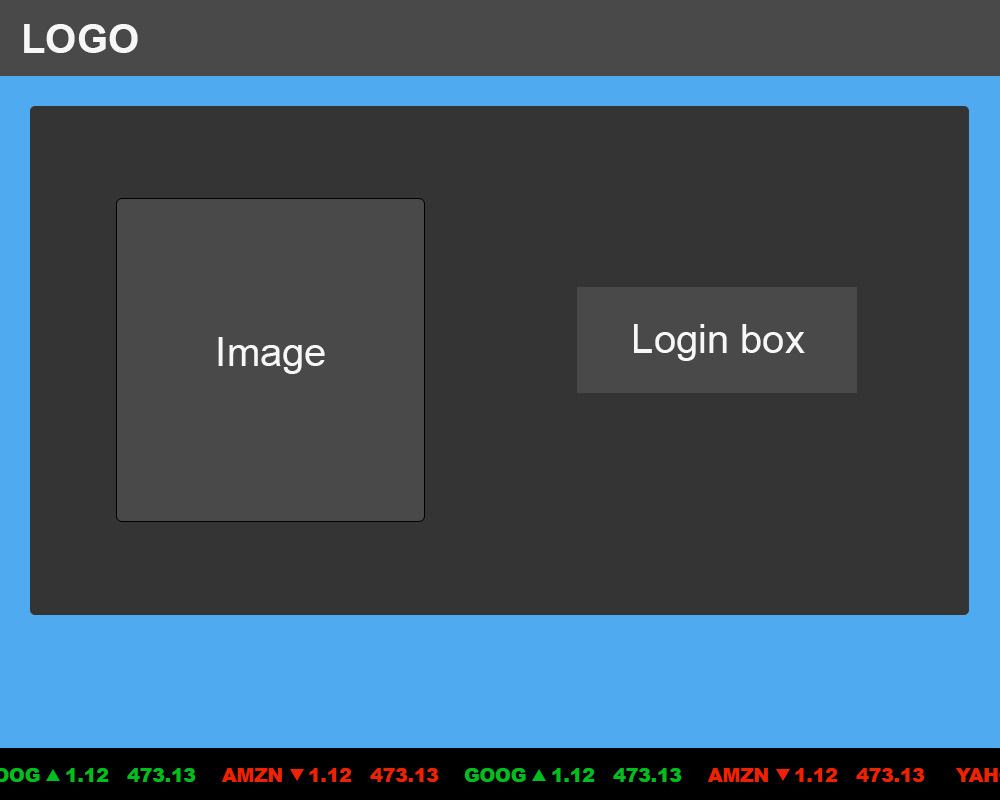
\includegraphics[width=5.5in]{./img/mock/loginmock.jpg}
\caption{Basic on screen requirements of login page}
\label{ui:mockup}
\end{figure}


% Chapter 3
% Include Functional Requirements Spec
% In this chapter discuss functional requirements
% This is worth a lot so let's nail it
\chapter{Functional Requirements Specification}


% Who has a stake in the project?
% IE prospective users, possibly the finance
% backend people, possibly companies...
\section{Stakeholders}

The target demographic for the software described tends to be centered on students and
first time investors. That being said, it is likely to see the software expand to take
a large role in both university and pre-university classrooms, as a means of teaching
general financial concepts. It would not be unlikely to see the game further expand to
a larger range of users than other similar software due to increased functionality,
addition of achievement and leaderboards, and ability to join with or without league
functionality. Specifically, the addition of achievements leaves the user with the
desire to return and spend additional time trading on the software.\\

The league will be a free service with the intention of eventually moving to a
subtle-advertisement platform which will have no impact on the user. Once a
substantial enough user-base is generated, it will not be unlikely to see
advertisements begin to commence in order to bring revenue to the company. As a free
service (with eventual advertisements) we expect the platform to attract the greatest
number of users, and due to increased functionality, keep said users on the platform
for the greatest amount of time. The software is targeted not only at students and
potential investors, but at nearly everyone who desires to gain a greater understanding
of the financial industry as well as those who would simply like to practice trading
before executing in the real market.\\
 % no typos here...

% Who are some actors and what are their goals?
% I'm filling this from Nick's use cases
% but there could be even more
% Probably include a new file 
\section{Actors and Goals}

\subsection{Guest}
A visitor to the website who has either not logged in or just a simple visitor
\begin{itemize}
\item[--] Register and create an account using OpenID/OAuth2
\item[--] View the latest trades
\end{itemize}

\subsection{Investor}
A user who has an account in our servers and is logged in to their account
\begin{itemize}
\item[--] Research the latest updates in the market
\item[--] View their portfolio
\item[--] Execute orders of any kind
\item[--] Join/create a league
\item[--] Take part in competitions
\end{itemize}

\subsection{League Administrator}
Manages the leagues that they have created
\begin{itemize}
\item[--] Can set league to be public/private
\item[--] Set the rules for the league
\end{itemize}

\subsection{Database System}
Holds the information for the accounts of all users
\begin{itemize}
\item[--] Insert information as accounts are created
\item[--] Push data back to views about users/events
\item[--] Store new data about about users/events
\end{itemize}

\subsection{Financial API}
Gives the stocks in our database up to date prices
\begin{itemize}
\item[--] Fetch real world information and update our database accordingly
\end{itemize}

\subsection{Site Administrator}
Manages the overall website
\begin{itemize}
\item[--] Ensure fair competition between leagues/players
\end{itemize}

\subsection{Browser}
The middleman between user and system
\begin{itemize}
\item[--] Present data to the user
\item[--] Retrieve data from the user
\end{itemize}

\subsection{Yahoo! Finance}
The unit that knows about current financial statistics
\begin{itemize}
\item[--] Retrieve data about stocks
\end{itemize}

\subsection{Queueing System}
A subsystem for scheduling orders so as not to block user
interactions.
\begin{itemize}
\item[--] Place orders to be executed or canceled asynchronously
\item[--] Schedule events and mailings for system
\end{itemize}


\iffalse
\begin{figure}
\centering
\includegraphics[width=5.5in]{./Diagrams/UseCaseDiagram.png}
\caption{This graphic illustrates the relationships between the core actors of our platform.}
\end{figure}

% This is for the use cases
% These take up a lot so should be in another file
\section{Use Cases}

\input{./tex/fulldress}

\section{System Sequence Diagrams}

NEED DIAGRAMS FOR THIS SECTION!!!!!



In the following sequence diagrams, we describe exactly the interactions between the key
actors our system. It is important to note that most of the interaction between the
user and system is facilitated by the browser. The user, through filling forms and button
clicks, instructs the browser which requests to make to the system.
In turn, the system communicates with the database to request the desired data,
takes any required actions, and delivers the data to the browser for presentation to the user. \\


UC-1 – Register/create an account
When the user navigates to the login/ register accounts page, this use case
is triggered. The system makes it necessary to have an account before using
Paramount Investments leagues. The System then takes the information that the
user has input and sends them to the database, which then sends it back to the
system to display on the screen to the user. If the system finds that the user that is
registering with the same credentials as an existing account, the system throws up
an error appropriately.\\

UC-2 – Create/ Join a league
This use case is triggered when the user navigates to the create league page.
The user requests the system to create a league, which then sends appropriate
data to the database. Once the data is stored successfully, the database sends a
confirmation back to the system, which then displays an appropriate message to the
user. If the user wants to join a league, the user requests the system appropriately,
which then sends the data to the database regarding the right league and if
successful sends the confirmation to the user.\\

UC-3 – View Market Data
When the user navigates to the research stock page, this use case is triggered. The
user specifies to the system exactly what market data they would like to view. If
the user wants to research off the company’s website, then user will click on the
hyperlink present in the system. If the user wants to view the data through the
interface that Paramount Investment Provides, the system then pulls information
from the Yahoo Finance API and then sends it back to the system to display to the
user.\\

UC-4 – Manage Portfolio
This use case is triggered when the user goes to his/her own portfolio page. The
user navigates to the view portfolio page. The system then requests the database
to retrieve the user’s information. Once the database sends this data back to the
system, the system displays it to the user. The user is now free to modify aspects of
his/her portfolio. Once the user is finished modifying/updating their portfolio, the
system will send the changes to the database, which will then store the information
and save it.\\

UC-5 – Place a market order
This use case is triggered when the user goes to place a market order in the place
order page. The user selects a league to place the order into. The system then
displays the information to the user, who then requests to place a market order.
The system then queries to Yahoo Finance API to retrieve information about the
stock prices. The system then takes that information and processes it with what
the user wants to do. If the order is completed successfully, it is appropriately
displayed.\\

UC-6 – Take administrative Actions
This use case is triggered when the administrator of the website/ league wants
to take action. The system first checks if the user logging in has administrative
privileges in their respective group. If so, the system then looks in the database
to check for any logged conflicts. If there are unresolved conflicts, the database
returns them and then user can then view the conflicts. If there are no conflicts to
be resolved, then display so appropriately to the administrator/logged in user.\\

UC-7 – Manage League Settings
This use case is triggered when the manager of a league wants to change the league
settings. The system first checks to see if the user that is logged in, is the league
manager and if so, the grants the user privilege to change league settings. The user
then requests to change the league settings. The system retrieves the league data
and modifies it as the user has requested.\\



\iffalse
\begin{figure}
\centering
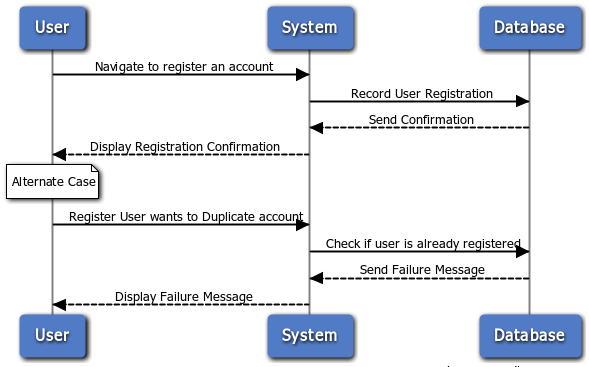
\includegraphics[width=5.5in]{./Diagrams/SystemSequenceDiagrams/uc1.png}
\caption{See UC-1 on page \pageref{UC-1}. When the user navigates to the league listing page, they invoke this use case. The user initiates a request to view all the public leagues and the system retrieves them from the database. Then, they are presented to the user who is given the option to join any valid league.}
\end{figure}

\begin{figure}
\centering
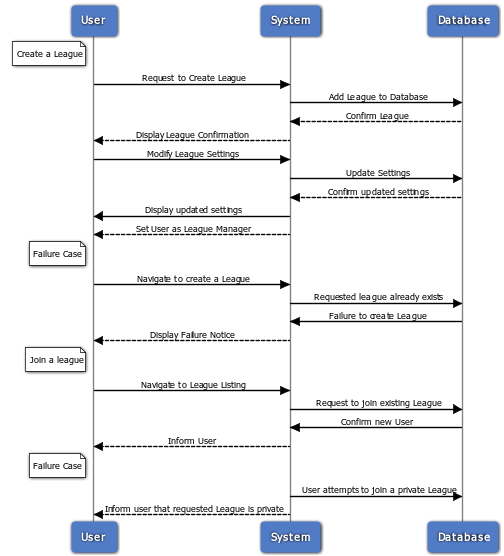
\includegraphics[width=5.5in]{./Diagrams/SystemSequenceDiagrams/uc2.png}
\caption{See UC-2 on page \pageref{UC-2}. This is sequence of events that occur when a league manager alters the league settings. The system fetches the current settings from the database and returns them to the browser. It also ensures that the user attempting this change is a league manager. Then, the user can initiate a request to change the settings which will be enacted out by the system. If the league manager changes the status of a user within the league, the system notifies that user.}
\end{figure}

\begin{figure}
\centering
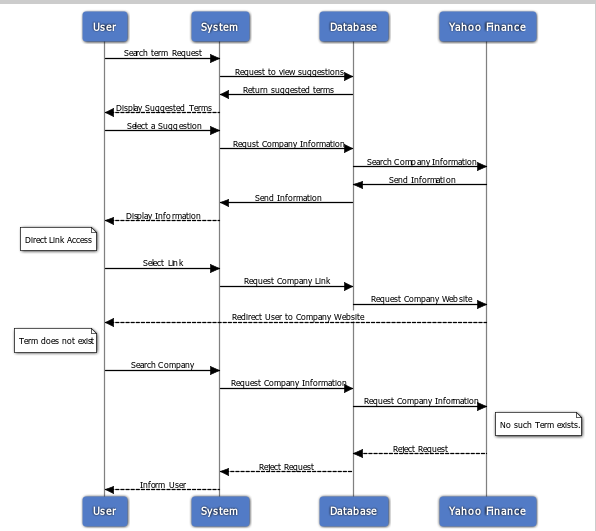
\includegraphics[width=5.5in]{./Diagrams/SystemSequenceDiagrams/uc3.png}
\caption{See UC-3 on page \pageref{UC-3}. When the user desires to research companies, this is the sequence that follows. The user is able to search and browse for companies. They can also get to a company's page through a direct link. Yahoo! Finance responds to requests and delivers data to our system which is then transferred to the browser and fills out a company profile.}
\end{figure}

\begin{figure}
\centering
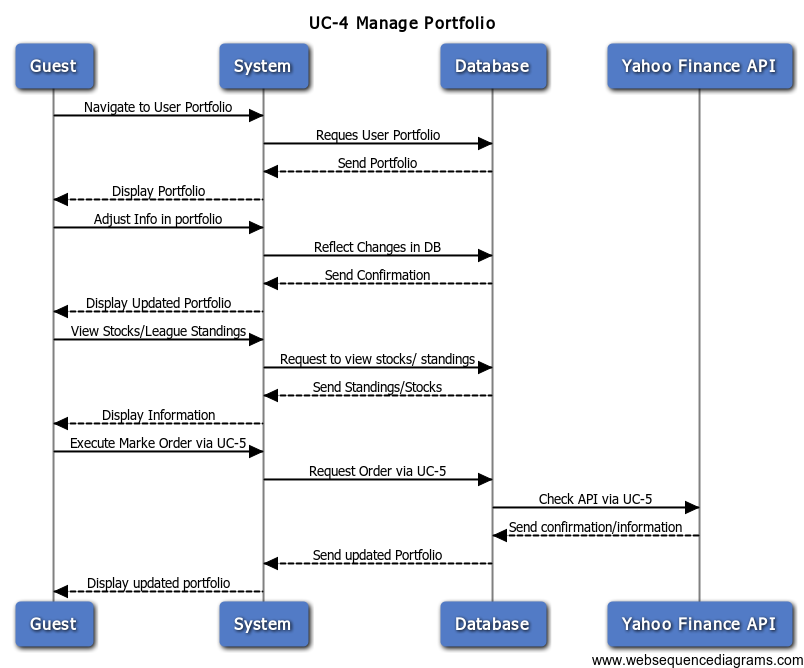
\includegraphics[width=5.5in]{./Diagrams/SystemSequenceDiagrams/uc4.png}
\caption{See for UC-4 on page \pageref{UC-4}. This sequence encompasses the bread and butter of our application--market orders. The user selects a league in which to place an order, fills out a prompt in the browser which then submits the request to the system. The system inserts the order into the database and enqueues it (the queuing system will be elaborated upon in a later section). Once the order resolves or expires, the database notifies the system and the user's portfolio is updated accordingly.}
\end{figure}

\begin{figure}
\centering
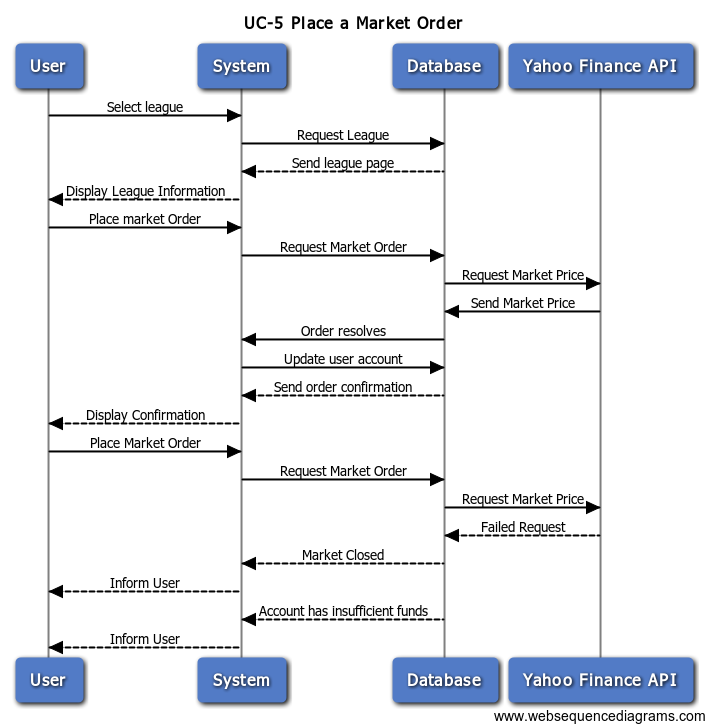
\includegraphics[width=5.5in]{./Diagrams/SystemSequenceDiagrams/uc5.png}
\caption{See UC-5 on page \pageref{UC-5}. This use case is relatively straightforward. The user browses to a league member's portfolio, and the browser submits a request to the database for that portfolio's inormation.}
\end{figure}

\begin{figure}
\centering
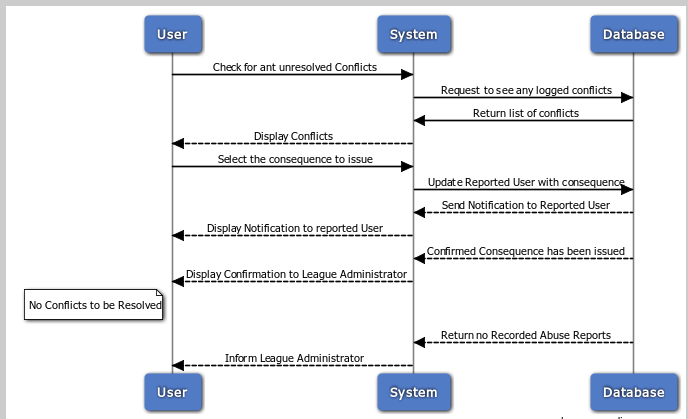
\includegraphics[width=5.5in]{./Diagrams/SystemSequenceDiagrams/uc6.png}
\caption{See UC-6 on page \pageref{UC-6}. Another simple use case. The user simply navigates to the tutorial page, which is populated by the system.}
\end{figure}

\begin{figure}
\centering
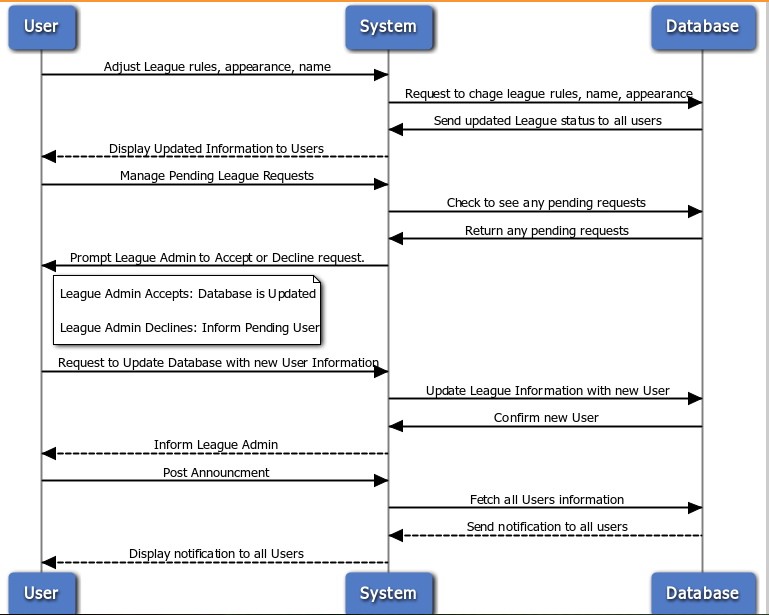
\includegraphics[width=5.5in]{./Diagrams/SystemSequenceDiagrams/uc7.png}
\caption{See UC-7 on page \pageref{UC-7}. When a site administrator navigates to observe any outstanding abuse reports, this flow of events is initiated. The database delivers all outstanding reports to the system which then populates them in the browser. If the administrator decides to take an action, the status change is reflected in the database, and the system notifies the user of whatever action was taken against them.}
\end{figure}
\fi

\fi


% Chapter 4
% Include UI Specification
\chapter{User Interface Specification}
\label{uispec}
% This section contains mockups, descriptions,
% and explanations, lots of graphics
\section{Preliminary Design}

The user interface (UI) for Paramount Invesments Leagues will act as a command center
for users to interact with their portfolio, leagues they are a part of, and conduct
research on potential orders. More specifically, the command center will act as the
primary; but not the only; view for users to interact with the system.  The command
center will provide a snapshot of the users current portfolio and its value, their
global rank, a dash to perform market orders, a news feed, and a graphing dash in order
to quick analysis of stock performance.  The UI will persist a users global rank across
all views as well as a ticker of current trades being placed through the Paramount
Investment League.\\

The UI should be lightweight so as not to burden our more restrictive target platforms
of mobile and tablet.  The colorscheme will be chosen to be easy on the viewer, though
this is subjective, the colorscheme will be a basic pallet of grey/black/white/blue,
tending toward pastel and web supported colors.\\

The UI will be built on top of Twitter's open source Bootstrap CSS\cite{wiki:boot}
framework to help
facilitate deleriving content to the three target platforms, desktop, mobile, and tablet.
Bootstrap provides a mobile first design philosophy, but can be customized to target
specific platforms.\\

\subsection{Landing Page and Login}

Paramount Invesment League is designed around allowing users to easily begin using the
service, also know as "zero effort" resgistration. In order to accomplish this, the
system does not require the user to register a new user name/account with our system,
but instead piggybacks on OpenID\cite{wiki:open} and OAuth\cite{wiki:oauth} allowing users to
use their Google,
Facebook, Twitter, and other OpenID/OAuth accounts to login. You'll also notice that
upon initial visit, the header is empty providing no navigation, this may be relaxed in
the future to allow the user to explore some of the features of the website that don't
require user authentication such as stock research. (\em See figure 3.1 \em)\\

\begin{figure}
\centering
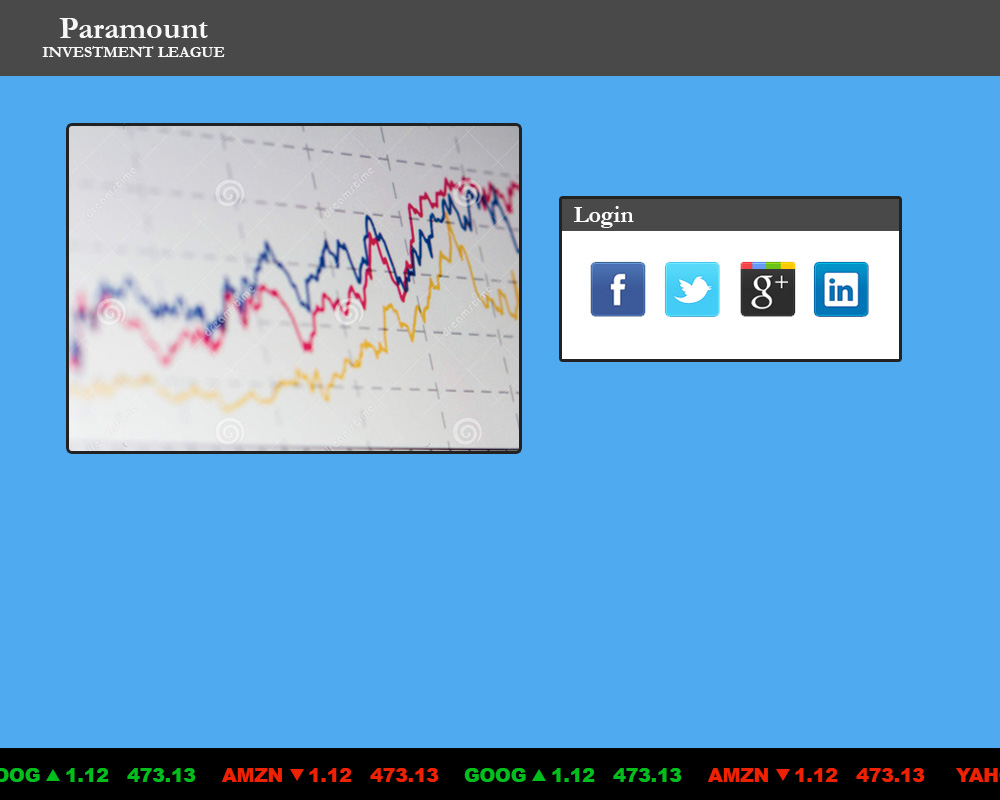
\includegraphics[width=5.5in]{./img/mock/login.jpg}
\caption{First iteration of Landing/Login page.}
\end{figure}

\subsection{Global Header}

The header (\em see Figure 3.2 \em)across the website will remain persistant across the
website once the user is logged into the system.  Navigation is done between essentially
4 views in the following order, My Portfolio, Stock, League, Leaderboard,.  These names
are placeholders and will most likely be My Portfolio, My Leauges, Leaderboards,
Analyze Assets. The 'My Leagues' and 'Leaderboards' will be turned into drop downs as
users expand into leagues to allow quick navigation.\\

The website name will also navigate to My Portfolio. The username will be replaced by the
users actual username, and below it will be the users global rank.  The rank will be
highlighted in red or green depending on whether they have improved their position on the
day, or it has declined.  It will also indicate how many spots they have moved.\\

\begin{figure}
\centering
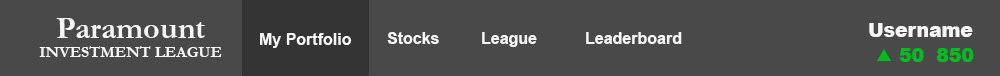
\includegraphics[width=5.5in]{./img/mock/topbar.jpg} %change with header
\caption{Preliminary design for a global header. This users is up 50 spots for the day.}
\end{figure}

\subsection{Global Ticker}

One interesting feature of Paramount Investment Leagues will be its active ticker at the
bottom of the website.  This ticker will be seen in all views, including the Landing Page
once there is enough volume to keep the ticker full.  The ticker serves two goals, one for
new users, and one for existing users.  The first goal is to entice new users to
participate by demonstrating that the app is being widely used. The second goal is to give
a snapshot to existing users of assets that are "on the move" so that they can attempt to
remain competetive. The ticker can be seen at the bottom of all the figures.\\

\subsection{My Portfolio}

The 'My Portfolio' (\em see Figure 3.3 \em) view of the  website will act as the command
center for a user wanting to get news about companies/assets in their portfolio, perform
an order, or conduct quick graphical anaylsis of assets in their portfolio and compare
them to any other asset available for trade through the platform.\\

More importantly, it provides a snapshot of the users portfolio including a scrollable list
of all the assets inside the portfolio and a summary of said assets.  In the future, assets
will be 'clickable' and will take the user to a summary page of that asset, but that is not
planned for the initial 2 iterations.\\

\begin{figure}
\centering
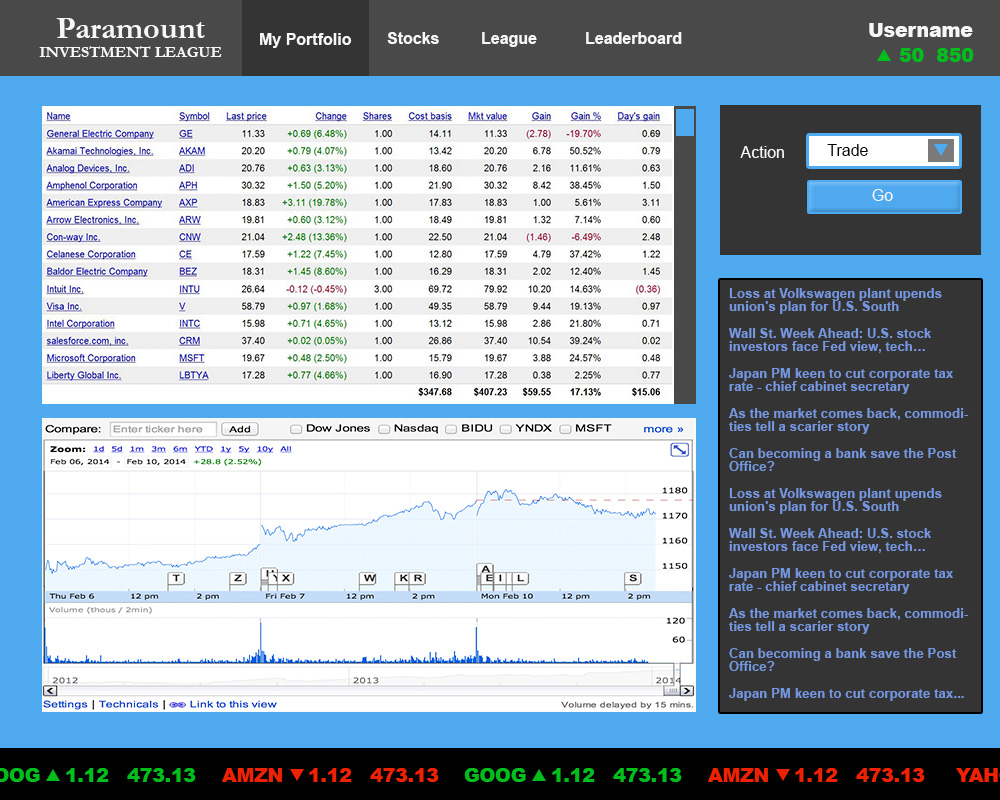
\includegraphics[width=5.5in]{./img/mock/portfolio.jpg}
\caption{The preliminary design of the 'My Portfolio' view.}
\end{figure}

\subsection{Leagues}

The 'League' (\em see Figure 3.4 \em) view will present a user that isn't a part of a league
the ability to create a new league of join an existing league.  Not shown in
\em Figure 3.4 \em is the view that a user who is a part of a league.  This view will still
persist the join/create dialogues, but will also present a list of all the leagues that user
is a part of, their rank within said league, and their movement within said league.\\

\begin{figure}
\centering
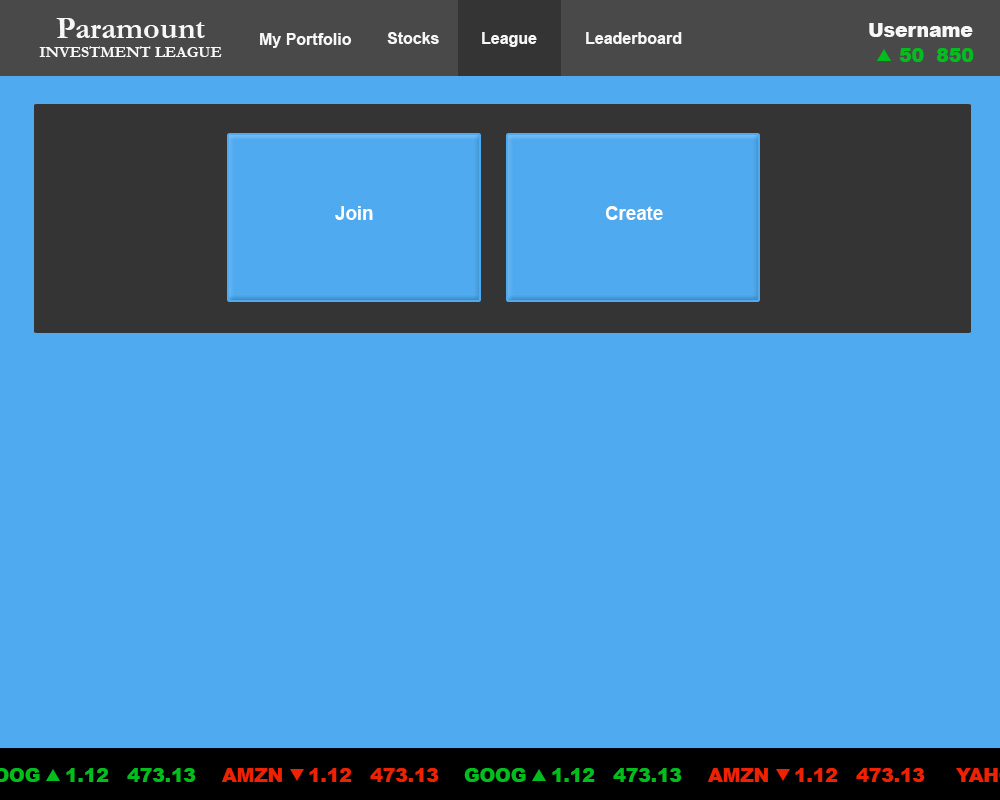
\includegraphics[width=5.5in]{./img/mock/league.jpg}
\caption{This is the league creation/join view. This would be the view presented to a user
that is a part of no league yet.}
\end{figure}


\subsection{Leaderboards}

The 'Leaderboards' (\em see Figure 3.5 \em) view will present the user with a partial view
of the full leaderboard for a given league, or for every user.  It will show their rank,
their movement, the value of their portfolio as well as the same stats for all other users
around them.  The view will be scrollable if there are more records then can be displayed,
and will center the user in the middle of the view unless they are at the top or bottom
of the board.\\

\begin{figure}
\centering
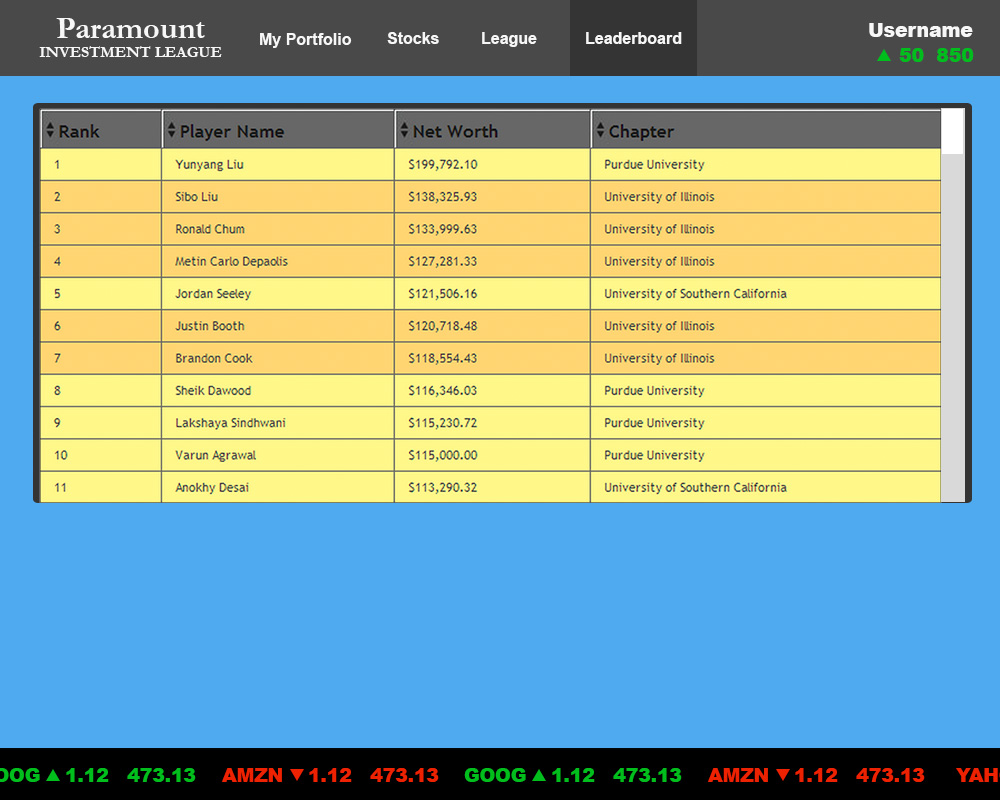
\includegraphics[width=5.5in]{./img/mock/leaderboard.jpg}
\caption{Here is the leaderboard view which will be the same for both leagues and global
leaderboards. This view represents a global leader board.  The colorscheme of this view
here is incomplete and will fall inline with the remainder of the site.}
\end{figure}

\subsection{Asset Analysis}
The 'Stocks' view (\em see Figure 3.5 \em) will be renamed to more align its function
with its name, which is to analyze assets. It will a more in depth way of anaylzing an
asset versus what is available in the 'My Portfolio' view.  There will be a news feed
at the bottom of assets that you are searching for. There will also be a more formal
analysis of asset data presented including P/E ratio, 52 week range, Volume, EPS, etc.
This isn't shown in the figure, but will one-half to two-thirds of the space that
has been set aside for the news feed.\\

This is also one of the views and functionalities that has been identified to not require
the user to be logged in.  While it will not be availble to non-users in the intial product,
it can be made available in future releases.\\

\begin{figure}
\centering
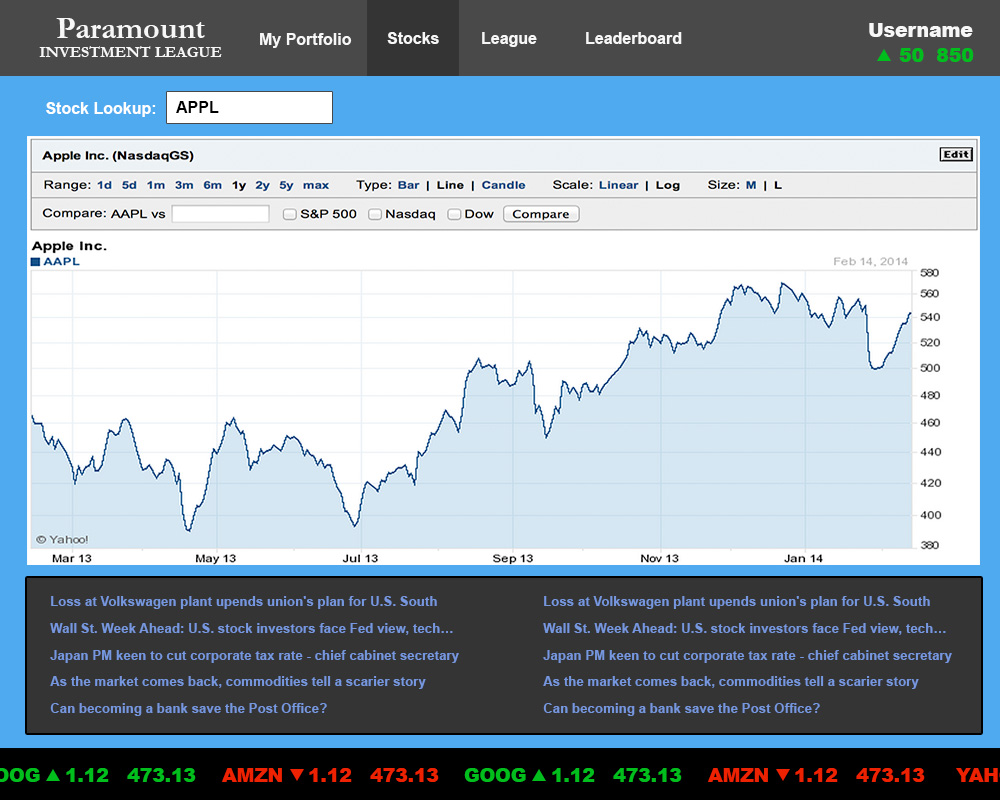
\includegraphics[width=5.5in]{./img/mock/stocks.jpg}
\caption{The preliminary view for asset anaylsis.}
\end{figure}


% This section contains lots of explanations
% of user effort and ease of access
% See Appendix A for examples to boost grade
\section{User Effort Estimation}

Several of the most common usage scenarios for Paramount Investment Leagues:\\

\begin{center}
\begin{tabular}{| l | l | l |}
\hline
\textbf{Usage Scenario} & \textbf{Clicks} & \textbf{Keystrokes} \\ \hline
Login \& Register & 2-3 & 0-1 \\ \hline
Place an Order & 4-6 & 2-12 \\ \hline
Join a League & 3-4 & 0-50 \\ \hline
Create a new League & 6-7 & 11-100 \\ \hline
Analyze Asset & 2 & 2-5 \\ \hline
View Leaderboard & 2 & 0 \\ \hline
\end{tabular}
\end{center}

\subsection{Login \& Register}

Assume the user has come to the domain and wishes to Login if already registered, or
register if already a user:\\
\begin{itemize}
\item \textbf{Navigation: }
\begin{enumerate}
\item Click on OpenID icon (Google, Facebook, Twitter, etc).
\item Click on your account (optional for multiaccounts).
\item Click on login, or hit enter.
\end{enumerate}
\end{itemize}

\subsection{Place an Order}

Assume the user has already logged in and they wish to place an order:\\

\begin{itemize}
\item \textbf{Navigation: }
\begin{enumerate}
\item Navigate to 'My Portfolio', 0-1 clicks.

\end{enumerate}
\item \textbf{Data Entry: }
\begin{enumerate}
\item Select order type from drop down, 2 clicks
\item Click textbox to enter asset name. 1 click
\item Enter assets name eg: 'G', 'O', 'O', 'G', 1-4 keystrokes
\item Press tab to specify number of shares, 1 keystroke (user could also execute 1 click)
\item Enter the number of shares, 1-7 keystrokes
\item Click execute, 1 click
\end{enumerate}
\end{itemize}

\subsection{Join a League}

Assume that the user wishes to join a league and is logged in:\\

\begin{itemize}
\item \textbf{Navigation: }
\begin{enumerate}
\item Click on League, 1 click
\item Click on Join, 1 click
\end{enumerate}
\item \textbf{Data Entry: }
\begin{enumerate}
\item Click on a League, or enter its name, 1 click or up to 50 keystrokes
\item Click on confirmation dialogue, 1 click
\end{enumerate}
\end{itemize}

\subsection{Create a League}

Assume that the user wishes to create a league and is logged in:\\

\begin{itemize}
\item \textbf{Navigation: }
\begin{enumerate}
\item Click on League, 1 click
\item Click on Create, 1 click
\end{enumerate}
\item \textbf{Data Entry: }
\begin{enumerate}
\item Enter its name, 1-50 keystrokes
\item Select ruleset from dropdown, 2 clicks
\item Fill in parameters, 1-2 clicks and 10-50 keystrokes
\item Click on confirmation dialogue, 1 click
\end{enumerate}
\end{itemize}

\subsection{Analyze an Asset}

Assume that the user is logged in and they want to start an in depth analysis of an asset:\\

\begin{itemize}
\item \textbf{Navigation: }
\begin{enumerate}
\item Click on Stock, 1 click
\end{enumerate}
\item \textbf{Data Entry: }
\begin{enumerate}
\item Click on the textbox for entering an asset name, 1 click
\item Enter an asset name, 1-4 keystrokes
\item Hit enter, 1 keystroke
\end{enumerate}
\end{itemize}


\subsection{View Leaderboard}

Assume that the user has logged in and wants to veiw a leaderboard:\\

\begin{itemize}
\item \textbf{Navigation: }
\begin{enumerate}
\item Click on Leaderboard, 1 click
\item Click on Select Legue/Global, 1 click
\end{enumerate}
\end{itemize}



% Chapter 5
% Effort Estimation ***New***
%\include{./tex/effortestimation}

% Chapter 6
% Domain Analysis
\chapter{Domain Model}

% Preface the high-level organization of the domain
\iffalse
At its highest level, Capital Games consists of a few subsystems
working together and coordinated by an internal controller. The
end user interacts with the application through either a web browser
or by directly submitting HTTP requests to the server. These actions
are equivalent because user actions are translated into RESTful actions
and interpreted equivalently by an appropriate RESTful controller. \cite{wiki:restful}
Once a controller is invoked, it consults the 
internal subsystems before responding to the request. Each of the 
subsystems can be identified by the purpose they serve in relation
to the application. 

% Concept Definitions
\section{Concept Definitions}

\subsection{Database}
By its nature as a data-driven site, data persistence
is core to Capital Games. Therefore, a database subsystem is necessary. 
A challenge often encountered when using databases in an application is
the translation of database-native datatypes to the more varied datatypes
employed by dynamic applications. \cite{wiki:orm} To simplify this,
Capital Games uses the ActiveRecord object-relational mapper to abstract
the logic between the database and the system as a whole. Only privileged portions
of the system have access to the database. This maintains the safety of the
data while also allowing it to be manipulated more precisely. Per the convention
of MVC-style application style architecture 
% insert reference here for later chapter
(upon which we base our application, described in more detail later), these 
are known as the Models. The database is explored in more detail in the Data Structures section.

\subsection{Finance API Adaptor}
The data for the application comes from a third party source, Yahoo! Inc. Yahoo!
provides both nearly-real-time and historical data on most U.S.-traded stocks.
Yahoo! exposes this data through a web API service in which a party can make
up to several thousand requests against Yahoo!'s databases daily. The party
simply enters arguments into an HTTP request which is interpreted by Yahoo!
as a database search, runs the query, and returns the results in CSV format. \cite{gummy}

In order to interact with the web service, we employ an adaptor plugin which
translates between the various syntaxes used by Yahoo! and our own system.
Any and all parts of the application which require access to a live data-stream
invoke the Finance Adaptor subsystem, which in turn queries Yahoo!. This
modularity enables multiple subsystems of the application to have access to live data
when necessary.

\subsection{Queueing (Asynchronous Task) System}

Fundamentally, Capital Games is about placing trading orders for various stocks. 
Though the simplest type, market orders, are executed almost immediately after being 
placed, stop and limit orders may not be executed for quite some time. \cite{inv:market}
\cite{inv:stop} \cite{inv:limit} This begs the question of how to perform a trade
at some undetermined time after the order is placed. 
Upon further inspection, a few other functions of the site depend on a similar capability.
In order to update the user portfolio database regularly or send out newsletters, the system 
must be able to asynchronously execute certain tasks. Enter a Queueing System.

Whenever a task needs to be performed asynchronously, the task is entered into a 
designated portion of a Redis database, configured as a queue. Background "workers" 
(processes) perform tasks as they arrive. Tasks can also be scheduled to occur at specific
times or intervals. In this way, everything from polling the datastream for stock updates
to performing scheduled updates and e-mails can be coordinated by a single system.

\subsection{Views Generator}

Finally, when all data have been collected and a response needs to be rendered, those data
are delivered to a subsystem which dynamically generates the content
which are served up to the end-user. The Views Generator contains various modules which
simplify translating the data to web-standard HTML and Javascript.

\subsection{Mailer System}

Capital Games is designed to periodically alert users as to their portfolio performance.
This is performed by the Queueing System in conjunction with the Mailer system.
The framework we employ natively contains a robust mailing system called Action Mailer,
which generates content dynamically at runtime. \cite{action:mailer} This allows us to perform calculations
on leagues and then include that into emails, in addition to raw data.

%\begin{itemize}
%\item \textbf{Users}: Every end-user of the application needs both a private and
%public facing identity on the site.
%
%\item \textbf{Site Administrators}: The site needs a few global administrators
%who can delete posts and ban users which are innappropriate, as well
%as perform several maintenance features.
%
%\item \textbf{Leagues}: Every end-user is participating in one or more leagues.
%
%\item \textbf{Investors}: Because an end-user can participate in multiple leagues,
%and each instance of the user can have a separate amount of money, margin,
%etc., it is necessary to maintain a separate identity for each of these 
%instances -- \emph{investors}.
%
%\item \textbf{League Manager}: Every League should have a superuser who is 
%able to invite other players, perform moderation, and change settings.
%\end{itemize}
%
%Although not actors themselves, from UC-4 (page \pageref{UC-4}) and UC-5 
%(page \pageref{UC-5}) it is apparent that end-users are implicitly 
%requesting and manipulating data for their orders and portfolios. These,
%too, become part of the application domain.
%
%\begin{itemize}
%\item \textbf{Orders}: When an \emph{Investor} places any type of order, it
%needs to be tracked. 
%\item \textbf{Stocks}: Whenever an Investor is tracking the performance of a
%stock, those data need to be stored locally. Stocks is a unified 
%data object to contain those data.
%\end{itemize}
%
%One of the actors at the back end of UC-3 (page \pageref{UC-3}) and UC-4
%(\pageref{UC-4}) was the Financial API, responsible for accessing the 
%market data stream. 
%
%\begin{itemize}
%\item \textbf{Financial API}: This module presents an interface for requesting market
%data, both live and historical. 
%\end{itemize}
%
%Upon further analysis, it becomes apparent that the domain model is missing
%functionality responsible for asynchronously executing jobs. This is another
%core feature of the site, without which Stop and Limit Orders could not 
%be placed.
%
%\begin{itemize}
%\item \textbf{Queueing System}: Many interactions need to be performed asynchronously,
%such as the execution of Stop and Limit Orders and the delivery of e-mail 
%updates. This module encapsulates the functionality of creating, maintaining,
%and executing jobs which need to be performed asynchronously.
%\end{itemize}
%
%Finally, we need an abstraction for the part of the system which invokes and operates
%upon the rest as a collective.
%
%\begin{itemize}
%\item \textbf{Controller}: The Controller is the model which receives requests from 
%the end-user, interprets them, invokes other models and modules accordingly, and 
%returns the response (when applicable).
%\end{itemize}
%
%
%% Association definitions between actors
\section{Association Definitions}

As indicated in Figure~\ref{domainModel2}, there are 6 components which are core
to our system: Controller, Views, Models, Finance Adaptor, Queueing System, and
Mailer.

The Controller acts as the single point-of-entry for all user interactions. It
interpretes requests and accordingly accesses the Models, the Finance Adaptor,
and the Queueing System, before delivering the necessary data to the Views
Generator. By definition, the Controller is the most prviliged system component.

The Queueing System is possibly more privileged than the Controller. It has a great deal
of autonomy, functioning without the Controller and being able to invoke other systems
on its own. Compare this to the Controller, which is only invoked upon requests from
a user. The Queueing System communicates with Models, the Finance Adaptor, and the 
Mailer as necessary to perform its tasks.

Conversely, the Views Generator is the least privileged subsystem. It cannot
externally communicate and only responds to to the actor which called it.

The Finance Adaptor, Mailer, and Models are each afforded limited privileges, in that the
Models and Mailer need to communicate with the database and Views, respectively, 
while the Finance Adaptor needs to communicate with external data sources through the Internet.
They each respond directly to requests from the componenets which invoke them.

\begin{figure}
\centering
\label{domainModel2}
\includegraphics[width=6.5in]{./img/domainModel2.pdf}
\caption{This high-level overview of the domain model of our application shows the 
separation between the external actors User, Browser, and Yahoo! Finance, as well as
how the internal component subsystems relate to each other.}
\end{figure}
%
%% brief discussion of how the parts relate to each other
%Clearly, many of these models are interrelated. Below is a non-comprehensive
%list of associations between various types of models.
%
%\begin{itemize}
%\item \textbf{Controller}: The Controller interacts with the collective database layer, 
%as well as the other core modules.
%	\begin{itemize}
%	\item \textbf{Association}: Controller invokes the Database layer (and data contained therein)
%	\item \textbf{Association}: Controller invokes the Financial API 
%	\item \textbf{Association}: Controller invokes the Queueing System
%	\end{itemize}
%\item \textbf{Queuing System}: The Queueing System can almost be thought of as a 
%miniature, self-regulating Controller. It can invoke the Financial API and the 
%collective database layer.
%	\begin{itemize}
%	\item \textbf{Association}: Queueing System invokes the Financial API
%	\item \textbf{Association}: Queueing System invokes the Database layer
%	\end{itemize}
%\item \textbf{Database Layer}: The Database Layer stores data into data objects and then
%saves them to the underlying database. The Database Layer can perform limited checking
%and updating logic when invoked, but is not self-regulating. It contains models of
%several types of actors.
%	\begin{itemize}
%	\item \textbf{Users}: Represents end-users and their personal information
%		\begin{itemize}
%		\item \textbf{Inheritance}: Users is the parent class of Site Administrators
%		\item \textbf{Aggregation}: Users have many Investors (User-Instances)
%		\item \textbf{Composition}: Leagues have many Users
%		\end{itemize}
%	\item \textbf{Site Administrators}: A superclass of Users
%		\begin{itemize}
%		\item \textbf{Inheritance}: Site Administrators inherits from Users
%		\end{itemize}
%	\item \textbf{Leagues}: Represents simulation instances
%		\begin{itemize}
%		\item \textbf{Composition}: Leagues have many Users
%		\item \textbf{Composition}: Leagues have many Investors (User-Instances)
%		\item \textbf{Aggregation}: Leagues have many Orders
%		\end{itemize}
%	\item \textbf{Investors}: Represents User-Instances within Leagues
%		\begin{itemize}
%		\item \textbf{Composition}: A League has many Investors
%		\item \textbf{Aggregation}: A User has many Investors
%		\item \textbf{Aggregation}: An Investor has many Orders
%		\end{itemize}
%	\item \textbf{League Managers}: A superclass of Investors
%		\begin{itemize}
%		\item \textbf{Inheritance}: League Managers inherits from Investors
%		\end{itemize}	
%	\item \textbf{Orders}: Contains order data
%		\begin{itemize}
%		\item \textbf{Aggregation}: Leagues have many Orders
%		\item \textbf{Aggregation}: Investors have many Orders
%		\item \textbf{Association}: Orders are placed for Stocks
%		\end{itemize}
%	
%		In addition, there are a few interesting types of orders, namely:
%		\begin{itemize}
%		\item \textbf{Market Order}: Orders executed immediately
%		\item \textbf{Stop Order}: Orders executed after a certain price is exceeded
%		\item \textbf{Limit Order}: Orders executed strictly beyond a certain price
%		\end{itemize}
%	\item \textbf{Stocks}: Contains data on stocks held by Investors
%		\begin{itemize}
%		\item \textbf{Association}: Orders are placed for stocks
%		\end{itemize}
%	\end{itemize}
%\end{itemize}
%

% Attribute definitions
\section{Attribute Definitions}

Though the application is a whole is not entirely object-oriented,
and thus not all parts (ie the Controller) have true attributes,
the Models, Queueing System, and Financial Adaptor all do. 

Models possess basic attributes for the data they contain, such
as user names, email addresses, stocks possessed, etc. These are
contained in Figure~\ref{domainModel}.  Similarly, Orders to
be performed in the Queue have similar identifiers, as shown in 
Figure~\ref{queuestruct}.

Validation on the data saved by the Models layer is performed 
automatically by the object-relational mapper, which can enforce
data typing rules built into the database. This happens automatically.

Orders data is proxied through the database, and so its data is also
validated before being entered. Though a remote edge case is the 
possibility of an order being valid while placed but being invalidated
(for example by a stock no longer being on the market) while in the
queue, we do not consider it at this time.

The Queueing System utilizes entities called ``background workers''.
As the name implies, these are persistent entities which wait
for work in the form of queued tasks to hit the Redis database. When
this happens, the first available worker pulls the task from the queue.

The Financial Adaptor possesses a set of financial metrics, a brief
list of which is tabulated in Table~\ref{financeparams}. When
data is retrieved by the adaptor, it is tabulated with some of the
parameters shown in the table. 


\begin{figure}
\label{queuestruct}
\centering
\includegraphics[width=6.5in]{./Diagrams/ComponentModels/BackgroundProcessStructuralModel.pdf}
\caption{The structural model of the Resque Queueing System. Market Orders to be placed are 
bundled as Orders and served to the queue to be processed every few minutes. Newsletters are 
performed daily and bundled and served every night. Background workers wait for updates to
the Redis database and upon seeing a valid task, pull it and begin processing.}
\end{figure}

\begin{table}
\label{financeparams}
\centering
\renewcommand\arraystretch{1.5}
\begin{tabular}{|c|c|c|c|}
\hline
Ticker & Name & Date & Time \\
\hline
Change \% & Previous Close & Open & Volume \\
\hline
Day High & Day Low & Day Range & Ticker Trend \\
\hline
Bid & Ask & Average Daily Volume & Price-to-Earnings Ratio \\
\hline
\end{tabular}
\caption{These are some of the data that Yahoo! Finance provides upon request, and which the adaptor we employ
can convert.}
\end{table}
%
\fi
%
%It is clear from the domain model abstraction above that the Database Layer
%models have many noteworthy attributes, and are heavily state-based. However,
%the Financial API has no state, and is simply an aggregation of functionality.
%Likewise with the Controller. Therefore, attributes are only elaborated on for
%the Database Layer. 
%
%\begin{itemize}
%	\item \textbf{User}
%		\begin{itemize}
%		\item Name: String
%		\item E-mail: String
%		\item Password: String
%		\item Admin: Bool
%		\item Banned: Bool
%		\end{itemize}
%	\item \textbf{Investor}
%		\begin{itemize}
%		\item Manager: Bool
%		\item League ID: Integer
%		\item User ID: Integer
%		\item Capital: Double
%		\item Margin: Double
%		\end{itemize}
%	\item \textbf{League}
%		\begin{itemize}
%		\item Start Date: Date
%		\item End Date: Date
%		\item Capital: Double
%		\item Margin: Double
%		\item Commission: Double
%		\item Privacy: Bool \footnote{To simplify joining private leagues, 
%			we allow that whenever a User is ``invited'' to join one,
%			an \emph{Investor} is created for them within that league, 
%			granting immediate access.}
%		\end{itemize}
%	\item \textbf{Orders}
%		\begin{itemize}
%		\item League ID: Integer
%		\item Investor ID: Integer
%		\item Time Ordered: Date
%		\item Time Executed: Date
%		\item Ticker: String
%		\item Order Type: String \footnote{Market, Stop, Limit}
%		\item Transaction Type: String \footnote{Buy, Sell, Short, Cover}
%		\item Quantity: Integer
%		\item Duration Valid: Date
%		\end{itemize}
%	\item \textbf{Stocks}
%		\begin{itemize}
%		\item Date: Date
%		\item Ticker: String
%		\item Price: Double \footnote{Any other interesting metrics can likewise
%			be stored here.}
%		\end{itemize}
%\end{itemize}
%
%The Queueing System itself is an aggregation of functionality
%present in the controller and operates on state data from the Database. However,
%it is still under active development, and so a model for it has not yet been 
%constructed. It could be one large, all-encompassing system, or (more likely)
%will be split off into individual subsystems.

% put some BS here...

% Traceability Matrix
% This section can be implemented at your discretion,
% and to the extent you desire. We were already
% kind of waived out of having one, but maybe include
% the derivations of the domain model from the use cases
% or at least why an MVC style works. No need to go into
% too much detail about MVC though, because there's an
% architecture report due next week anyway...
% \section{Traceability Matrix}

% Put the Domain Model Graphic here:

\section{System Operation Contracts}

% "Should be provided only for the operations of the fully-dressed
% use cases elaborated on in Section 3c for the operations identified
% in section 3d". 
% So not sure what to do about this...


\textbf{UC-1 Register/Create an Account}
\begin{itemize}
	\item \emph{Preconditions}
		\begin{itemize}
		\item (join) If a new user is visiting the Paramount Investments League website (guest), they must first register with either OpenID/OAuth2 account before joining/creating a league with Paramounts Investments.
        \end{itemize}
	\item \emph{Postconditions}
		\begin{itemize}
		\item After registration, the database is updated and logs the once previous guest, as an investor of Paramount Investments League.		
        \end{itemize}
\end{itemize}

\textbf{UC-2 Create/Join League}
\begin{itemize}
	\item \emph{Preconditions}
		\begin{itemize}
\item Investor must be logged into the Paramount Investments League website.
\item No more than one instance of the same League name can exist.
\item User hasn’t joined a league yet.
				\end{itemize}
	\item \emph{Postconditions}
		\begin{itemize}
\item Investor has joined a league
\item Database has been updated
\item League has been set with selected settings.
			\end{itemize}
\end{itemize}

\textbf{UC-3 View Market Data}
\begin{itemize}
	\item \emph{Preconditions}
		\begin{itemize}
\item Investor is logged in
\item Yahoo Finance is accepting inquiries.
			\end{itemize}
	\item \emph{Postconditions}
		\begin{itemize}
		\item None
		\end{itemize}
\end{itemize}

\textbf{UC-4 Manage Portfolio}
\begin{itemize}
	\item \emph{Preconditions}
		\begin{itemize}
\item User is logged into their Paramount Investments League account. 
\item Yahoo Finance is accepting inquiries. 
		\end{itemize}
	\item \emph{Postconditions}
		\begin{itemize}
\item Any adjustments made to the investors portfolio have been updated in the database.
\end{itemize}
\end{itemize}

\textbf{UC-5 Place a Market Order}
\begin{itemize}
	\item \emph{Preconditions}
		\begin{itemize}
\item User is logged into their Paramount Investments League account. 
\item Investor has enough funds in their account to place a market order
\item Yahoo Finance is accepting inquiries. 

		\end{itemize}
	\item \emph{Postconditions}
		\begin{itemize}
\item User profile is reflected with any change to funds or position.
\item Database has been updated with these changes.
		\end{itemize}
\end{itemize}

\textbf{UC-6 Take Administrative Actions}
\begin{itemize}
	\item \emph{Preconditions}
		\begin{itemize}
\item User is the site administrator
\item An issue/conflict occurs and needs to be resolved.
\item There are outstanding abuse reports.
		\end{itemize}
	\item \emph{Postconditions}
		\begin{itemize}
\item Conflicts/Issues have been resolved
\item The reported user has been notified of any actions taken against them.
		\end{itemize}
\end{itemize}

\textbf{UC-7 Manage League Setting}
\begin{itemize}
	\item \emph{Preconditions}
		\begin{itemize}
\item Initiating actor is the league manager. 
\item League Manager is logged into their Paramount Investments League account.
		\end{itemize}
	\item \emph{Postconditions}
		\begin{itemize}

\item Database is updated to reflect any changes  made to their account.
\item All users are notified of any changes made in their league. 
		\end{itemize}
\end{itemize}

\section{Economic and Mathematical Models}
\label{econmodels}
\subsection{Perfect Competition}

One of the prevalent concepts in the stock market is the economic concept of perfect
competition, which says that not any single participant has enough resources/power
to control the market.  To apply the concept of perfect competition to our project
we will need the following requirements:

\begin{itemize}
\item
Not one person can control the market or industries, segment, etc.
\item
Users can feel free to execute trades at their convenience without having to worry
about extra costs
\item
Every individual has access to same stock information as other investors
\item
The selling price is the same as the buying price.
\end{itemize}


In the real world, none of these requirements can be met, as there is always some
problem that prevents the market from being in perfect competition.  The following
are just some of the problems:

\begin{itemize}
\item
There are high net worth individuals/companies who have enough capital to change the
tide of a certain sector of the market.  If one of these individuals suddenly decides
to leave a particular market, the move may suddenly shift the market and effect other
investors in that market.
\item
In the real world, users typically don’t have direct access to stocks. They have a
broker (electronic or human) who they interact with, who then have direct access
to stocks.  Users can’t usually execute trades/buy stocks without worrying
about extra costs because of the commissions charged by brokers when trading
stocks.
\item
The world is not a fair place, and neither is the stock market. There are individuals
who because of the field that they work in, have much more insight into a particular
industry/stock.  These individuals then sell this information to potential buyers in
hopes that it gives them an edge in trading. This gives a huge disadvantage to those
that don’t have access to more information bout stocks.
\item
Lastly, in the real world, the selling price is never usually the same as the bid
price.  The Bid-Ask spread, the difference between the buying and selling price
tends to be greater than 0.
\end{itemize}

All these factors lead the stock market away from perfect competition.\\

How do we plan to fix these issues to ensure a near-perfect competition?

\begin{itemize}
\item
All investors start with the same amount of money, this way no one person by default
has more power than anyone else
\item
No commission will be charged when the trades are executed for any investor
\item
Insider trading will be avoided by standardizing the stock information across the board
\item
The ask-bid spread will be 0, so the selling price is the same as the buying price
\end{itemize}

Mathematical Model:

\begin{itemize}
\item
Stock Prices
\begin{itemize}
\item
There are no complicated mathematical models behind how the stock prices are
determined in our platform.  The market prices that are retrieved from Yahoo Finance
are the prices that are available to users in Paramount Investments
\end{itemize}
\item
Achievements
\begin{itemize}
\item
Achievements in Paramount Investments each have their own mathematical model.
There are no complicated algorithms behind how these achievements are attained.
If the user has met the required conditions for a certain achievement, then they
will be given that specific award.
\item
For example: Buy stocks whose P/E Ratio > 1
\end{itemize}
\end{itemize}



% Chapter 7
% Interaction Diagrams
%\include{./tex/interactiondiagrams}

% Chapter 8
% Class Diagrams and interface Specification

% Not needed in Report 3.1
%\include{./tex/classdiagram}

% Chapter 9
% System Architecture and System Design
\chapter{System Architecture and System Design}

\section{Architectural Styles}

In order to make the most efficient use of our software, we
will couple several known software tools and principles into
our design. The follow architecture types will be expanded in
detail to not only reflect general functionality, but also to
reflect functionality of the software as a whole. As explained,
each will play a crucial role in the success of our software and
will be largely derived from the necessities of the software.
That being said, architectural systems will include (and may be
expanded upon in the future) the Model View Controller,
Data-Centric Design, Client-Server access, and RESTful design,
with each architecture serving a small part of the whole result.

\subsection{Model-View-Controller}

The Model View Controller is a User Interface implementation method
which will separate the software into 3 specific groups; that is:
the model, view, and controller subsections. The view category is
typically limited to UI specific output, i.e. a webpage with stock
information. That being said, the model remains the core component
of the MVC method which holds all of the data, functions, and tools.
The controller simply takes the input and converts it into a command
for either the model or the view.\\

The MVC method is ideal for this particular software because it allows
the design to be broken down into smaller sub-problems. By splitting
into 3 parts, we can separate UI functions, from database functions,
and have all of them handled ultimately by the controller. Thus in
terms of fluidity of the design, adding in the MVC allows each to be
distinct and allows for the programming to be made far easier.

\subsection{Data-Centric Design}

Data is the fundamental backbone of Paramount investments.
Stored within our database, will be numerous bouts of data,
which will be necessary for all aspects of the software. The
database needs to contain not only data pulled from the Yahoo!
Finance API, but more importantly user specific data. Whenever
the user logs in, they need to have access to a personal host of
their own data. That includes but is not limited to complete
portfolio, leagues, achievements, leaderboard, and settings.
More importantly, the data needs to be stored in a way that it
can be accessed by multiple subsystems whenever necessary. So
in using this method, we can keep the data specific parts in the
software abstract and easily accessible.

\subsection{Client-Server Access}

The user will be constantly interacting with the interface.
All of the interactions are occurring, thus, on a client
server basis. The user remains the primary client, and as
such, constantly must interact with the other subsystems.
All of the infrastructure provided by Paramount Investments
will need to be accessed by the user. This ensures a smooth
communication between each of the parts of the MVC and between
client and infrastructure. Further, the infrastructure provided
by Paramount investments will be able to access infrastructure
of non-associative systems.

\subsection{Representational State Transfer}

As a software implementing a client server Access system,
a REST system is also inherently implied. The RESTful design
principles state that in addition to having a Client-Server
Access system, the system has a scalability of components,
that the interface is uniform, stateless, and cacheable.
Using this method will employ a smooth, modular set of code.
Using the interface specifications within the RESTful outline
allows both the user and the designers to have streamline
interactions with the interface. That is the user knows quite
clearly what he or she is doing when say a link is clicked on
a web page. The request is converted and sent out to the controller.\\

Importantly, the RESTful implementation can be implemented on
multiple levels. And as is desired, this system will be able to
work on Android and iOS as well as through standard web interfaces.
Thus a smooth transition between these mediums is incredibly
important. Thus whether a user places an order on his cell phone
or online, he should be able to experience a uniform experience
across all mediums. Using the RESTful system will help in this process.


 % done

\section{Identifying Subsystems}

Paramount investments aims to set its platform on multiple interfaces.
As such, subsystem identification becomes an integral part of initial
analysis of the software. On a thick layer, our platform exists with
a front-end system and a back-end system. But on a much deeper level,
we can see that, each of these subsystems can be broken down into
still greater detail. Front end systems typically involve user
interface, and object interactions with the user. Back-end will refer
to all database schema, implementation and interactions with relevant
hardware. Also included are non-associative items which are necessary
to the success of our system.\\

Front-end systems are formally plain. The user interface which displays
views and specific data to the user on multiple platform is included
here. That is, it will contain different mappings and specific
implementations for iOS and Android as well as natively for the Web.
The front-end system will have to maintain constant communication
with the back-end system to maintain consistency and retrieve data
regularly. It needs to be able to successfully communicate information
from commands given by the user and communicate them to the back end.
The back end system will retrieve necessary data and information and
return the data to the UI and user to project the page or information
requested.\\

Our back end system will be broken down further and is easily
considered the most important part of our infrastructure. Since
we are using the MVC framework, the back end system is to be broken
down into controller and database subsystems. Additionally, we will
have the financial retrieval system and queuing systems as previously
outline. Thus, the bulk of the command processing is handled by our
back-end subsystem.  The back-end system must not only communicate
among the subsystems within itself, but it must also communicate with
the front-end UI system to respond to commands and also communicate
with the non-associate systems as well.\\

Breaking down the subsystem further, we highlight the importance
of the financial retrieval system, and the queue system. The
financial retrieval system will communicate with Yahoo! Finance
to retrieve relevant information as requested by the controller
(whenever the controller receives an input from the front-end user).
The queuing system will handle other processes and largely
communication with non-associative systems. It will also be
involved in queuing and handling all back-end processes and
monitors to ensure that the correct commands are processed at the
correct time. The success of these modules, the success of the entire
back-end system, and the success of communication amongst the
systems will be crucial for the overall success of the software.

 % done

\section{Mapping Hardware to Subsystems}

The Paramount Investments League is contained on a MySQL
database server, which is stored on one machine. However,
the system as a whole is spread across several machines. The
system to be is divided into two separate sections: a front-end
side that is run on the client’s web browser of choice, and a
back-end that runs on the server side of the database. The front-end
is the main graphical user interface (GUI) between the system and
the client. The front-end is responsible for communication between
the GUI and the database for purposes such as confirming market
orders and updating an investors portfolio. These changes in the
front-end are reflected in the back-end side of the server. The
back-end will handle proper execution of market orders and will
updates users on each of their transactions.

 % done

\section{Persistent Data Storage}

The plan for data storage exists at the core of Paramount
Investments. Since so much of our software depends on
properly developed and updated data, it is of the utmost
important that our database schema represent accurately all
objects involved. That is, the data must accurately (at all
times) reflect all relevant user data, stock information,
ticker variables, league settings, achievements, leaderboards,
and all other relevant objects.\\

Paramount Investments will make heavy use of the relational
database MySQL. Relational databases are far more practical
for the needs of this particular software. That is, relational
databases consist of several indexed tables filled with
various object attributes. As can be viewed in the class
diagrams on the previous page, this is necessary for the
large quantity of objects which will be present in the
software. Tables will need to exist not only for user data
and settings such as log in and league profiles, but also
for stock and portfolio information. Further, these databases
need to be constantly written and rewritten to ensure
constantly updated and accurate information. Items such
as leaderboards, and information which will be able to be
viewed on each user’s portfolio need to constantly reflect
accurate data.\\

The data will be retrieved from the respective database table
in the form of a query. When a user inputs a command to retrieve
data, a query must be placed, the table searched, and the eventual
correct data value (or values) returned. For example if a user
requests his or her settings, it can query currently selected
settings and return those values to the UI and to the user. If
the user elects to make a change this will be sent back to the
database, updated and saved for further access later. The same
process can be mirrored and applied to all facets of the software.
Several tables will be used for varying data as has been outlined in the diagrams above. The success of the software is dependent on the values being returned accurately and in the most updated form at all times. Because of that, the database must receive a regular feed from the Yahoo! Finance API in order to constantly update and reflect data when queries are placed. In doing so, users will have constantly accurate views of their portfolio performance, leaderboards, achievements, stock tickers, and recent trades going on throughout the league and entire user base. It is in this way that the Paramount Investment software will distinguish itself from others and retain functionality and efficient realization of its ultimate goals and requirements.

 % done

\section{Network Protocol}

As is standard for software of this type, Paramount Investments
will uses the standard Hypertext Transfer Protocal (HTTP). HTTP
acts by structuring text which is uses hyperlinks to communicate
messages through text between nodes. While not necessarily unique
or particular to our situation, it is still important to note that
this will be the primary protocol between user and software
interface. More importantly, the HTTP protocol will be used not
only on web-based devices but also on Android and iOS devices as
well. From any of these mediums, the users can access various
webpages and links from the Paramount Investment website. They will
be able to access, through this protocol, all relevant stock,
portfolio, and relevant information through these pages and by
using the HTTP protocol.

\begin{figure}[h]
\centering
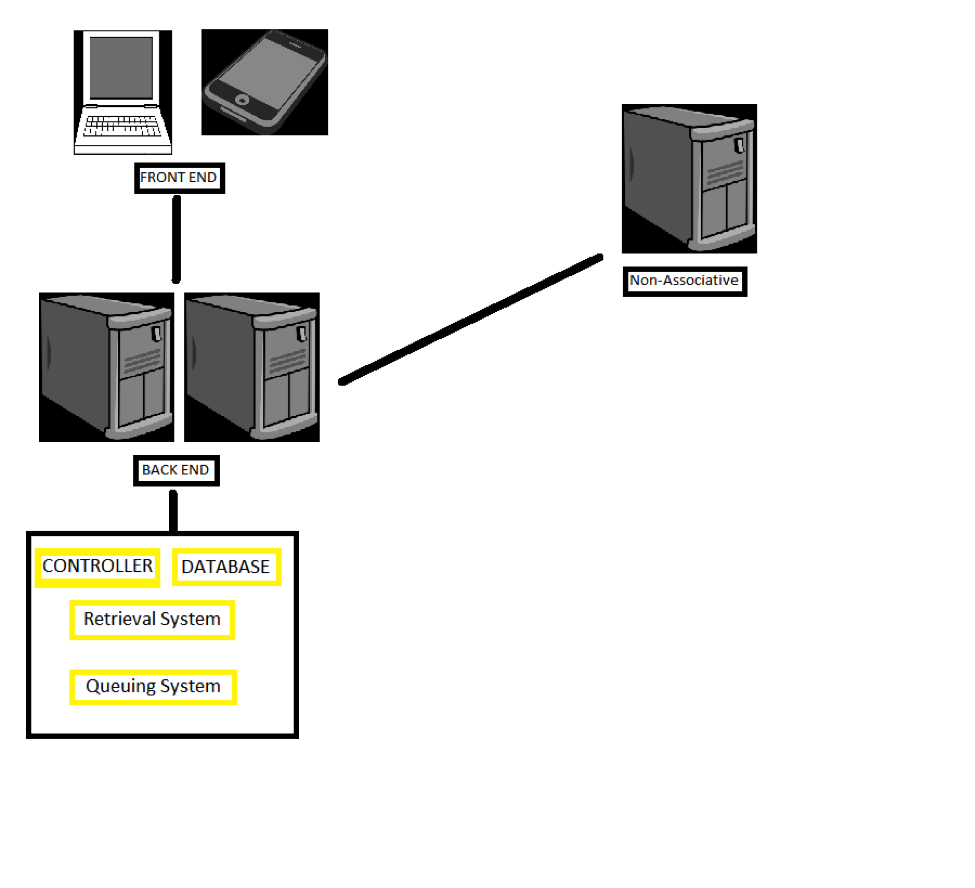
\includegraphics[width=7in]{./img/protocol.png}
\caption{Diagram of the network protocol.}
\end{figure}
 % done

\section{Global Control Flow}

\subsection{Execution Order}
In general, the implementation of the system at Paramount Investments
is for the most part, event-driven.  All the features that the system
has to offer must be triggered by some entity, whether it be the user
themselves or some other part of the system.  Overall, most of the
event-driven characteristic comes from the user end of the system.
Many of the functionalities (stock trading, portfolio viewing, league
joining, etc..) can only be triggered by the user.  There are however,
some event-driven functionality that are initiated by the system. When
the user places an order, it is processed and added into the database.
From here, the system initiates the process of checking the order and
then it uses Yahoo Finance API to retrieve market information about the
stock, obtain a quote and then actually process the order.\\

There is some functionality that have to be executed in a defined order.
Before the user starts investing, they must a few steps:
\begin{itemize}

\item[--]{Registration/creating an account: any user must register
within our website before joining a league.}

\item[--]{Join a league: any user must first join a league before
they can start investing.}

\item[--]{Achievements: any user must first complete the required
criteria before they can be awarded with the achievement trophy.}

\end{itemize}

However, on the whole, our system is still definitively an event-driven one.

\subsection{Time Dependency}
In general, the system at Paramount Investments is very much a real-time system,
but there are features that do not depend on time.  The real-time system is very
reliant on the stock market, which itself has certain times of operation.  As
the user is browsing the website, there are real-time timers that help the system
process information that it is receiving.

\begin{itemize}
\item[--]{Achievement Timer: This timer is used at the end of the day to check
for achievement specs for all the users.  Achievements/ rewards will then be
    dished out accordingly.}

\item[--]{Stock Market open and close: The stock market has a time interval
between when it’s open and when it is closed.}

\item[--]{Queuing system: the orders placed by users are placed into a queue.
Depending on market conditions, this can place high loads on the server.
To balance the server load, we must split the orders effectively.  The timer
in this system helps to check for unexecuted/ outstanding orders and then processes
them.}

\end{itemize}

\subsection{Concurrency}
There are sub-systems in our main system which have to be carefully thought of
due to concurrency.  The biggest of these is the queuing subsystem.  This produces
a concurrency issue because we have to make sure that no more than 1 order is being
inserted into the queue at any given time.  Likewise, we also have to make sure that
no more than 1 order is being dequeued from a given queue.  Other than this our system
really does not need any synchronization.  However, this may change as we are
implementing our system.

 % done

\section{Hardware Requirements}

The hardware requirements on the server side are the main
contribution to the operation of Paramount Investments League,
leaving the client-side with minimal requirements. In fact,
the only requirement of a client will that it runs a browser
that is capable of running a modern web browswer.

\subsection{Internet Connection}

In order for Paramount Investments League to use any of its core
functions (trading stocks, updating user portfolio, tracking
administrative actions, etc.), an internet connection is required.
Since most of the data being transferred is text (executable
instructions), a low band of frequency is required. Note that a
complete scalable analysis has not been performed on the system,
so a low band of frequency is based off of the needs of the current
website. For ideal performance, higher bandwidths of frequency
should be used in order to reduce any overhead. A network
connection between the server and the Yahoo Finance API is necessary
during trade hours (9:30am - 4:00pm Monday through Friday), otherwise,
no investors can perform a transaction.

\subsection{Disk Space}

The server must have adequate hard drive space to be able to
store all of the database information. All data being stored
is the sum of all program instructions for the system. 10 GB
of storage space should be sufficient for the system.

\subsection{System Memory}

Since this system is in active development, there is limited
concrete evidence that supports the overall performance of the
system. The system will load copies of database stored information
in order to operate over it. For better throughput, the memory
should be managed using a Least Recently Used scheme (LRU) in
order to keep the system memory populated with useful information.
A LRU scheme will release any bits of memory that haven’t been
accessed in a long time, and it will replace it with information
that is used more often. Also, any operations used on loaded
information will also use up system memory. A minimum of 512 MB
should be used for testing our system. In addition, as our user
based expands, it is obvious that the system memory will also
have to grow with it.

\subsection{Client-side Hardware Requirements}

The core hardware requirement on the client-side of the system
will be an internet connection. This is essential for the client
to be able to remotely connect to the server in order to access
the database. Without an internet connection, no client will be
able to use a web browser to visit the Paramount Investments League
website. In addition to an internet connection, and for a friendly
user experience, anyone on the client-side should have a functional
mouse and keyboard, as well as a graphic display to see their
portfolio. To display the Paramount Investments League website,
a screen with a minimum resolution of 800x600 pixels is adequate.


 % done


% Chapter 10
% Data structures used

\chapter{Data Structures \& Algorithms}

% In the DB we use tables because...
\section{Data Structures}

In the implementation of the system at Paramount Investments League, there will
be 3 main data structures in use.  These 3 data structures are a Queue,
ArrayList, and the HashMap.

\subsection{Queue}
The system at Paramount Investments league uses a queue data structure to
hold all the orders/transactions that users may place during in the system
during the day.  Because of the FIFO (First in First out) property of the queue
the orders that were placed first will the ones that are executed/processed
first.  This mimics the real world scenarios and will help capture part of the
essence of stock market trading.  At this stage in the implementation, we will
be trying to accomplish this using the interface provided to use by the Queue
Interface in Java.  One of the requirements we require of this queue is that it
be thread safe since there can be multiple users placing their orders at the
same time into the same queue.  If we find that there is a space limitation or
lack of thread synchronization of this queue implementation, we will make an
attempt to code the queue ourselves.

\subsection{ArrayList}
The system at Paramount Investments league will also be using an array data
structure to keep track of the positions that an investor might have in a single
stock.  In most case, investors will have only one position per stock but there
are scenarios where this is not true and the investor may have more than one
position in a single stock.  Because we are unsure of how many positions the
investor might want, we need to be able to account for this using a data
structure that has quick random reads but also has the capability to grow in
size without restriction.  This is achieved using the ArrayList class provided
in Java.  The ArrayList class has random read capability just like an array, but
it also has the capability to grow indefinitely just like a linked list.  Hence
we will be using the ArrayList to keep track of the positions per stock.

\subsection{HashMap}
The system at Paramount Investments League will be using a HashMap to keep track
of all the stocks that a user chooses to invest in for a given portfolio.  This
data structure needs to have quick insertion, delete, and read times.  We chose
the HashMap to accomplish this task because of the speed at which it is
possible to insert, delete, and access information in a HashMap.  Because there
are hundreds of different stocks, quick access to information is a necessity.
We plan to accomplish this task using the HashMap class in Java.

\section{Algorithms}

At the time of this report there is only one interesting algorithm that has been
designed and implemented.  We expect as the project progress for this section
to flesh out more and more, and include additional algorithms.

\subsection{A Method For Reducing API Calls in a Highly Concurrent Environment}

Our system relies on external API's\cite{wiki:api} in order to accomplish the
most central tasks, namely retrieving up-to-date stock data.  Since we are using
a free API, their are limits to the number of times that we can request
information from the API without having our IP address\cite{wiki:ip} blocked.
In order to limit the number of calls that are made, we need to cache the
results on our servers.\\

In order to accomplish this we wrote a service that is concurrent and maintains
a cache of stocks values on our server updating them periodically.  Here is a
brief overview of the algorithm:\\

\begin{algorithm}[H]
  \caption { Retrieve and Cache Stock Values }
$stockTicker \leftarrow$ End user does an operation that requires a stock value\;
$stock \leftarrow HashMap.get(stockTicker)$\;
\If { stock exists }
{
  \Return $stock$\;
}
Synchronize\;
\If { stock exists }
{
  \Return $stock$\;
}
$stockValues \leftarrow YahooAPICall(stockTicker)$\;
$stock \leftarrow new Stock(stockValues)$\;
$HashMap.put(stockTicker, stock)$\;
\Return Stock\;
\end{algorithm}

\vspace{5mm}

In order to make the above algorithm work in a Concurrent environment, we
synchronize\cite(wiki:sync) it in the critical section, that is, we only allow
one user at a time to add something to the HashMap.\\

In order to update the HashMap periodically, we run a background thread that
sleeps for some defined amount of time, then runs.  This background process,
builds an entirely new HashMap, and once complete, replaces the out of date
HashMap.\\


% Chapter 11
% User Interface Design & Implementation

% Not needed in Report 3.1
%\chapter{User Interface Design \& Implementation}

\section{Updated Pages}

At this time, there has been no discernible progress from the UI mocks that
were done in report 1.  That said, we expect there to be many small, but
substantial tweaks made to the final site once we begin doing user interaction
studies.  We also expect there to be minor changes made for the first
demonstration, but this hasn't been implemented or finalized yet.\\

\section{Efficiency of the Views}

One thing that we need to concentrate on is ensuring that the website is fast
for all users no matter what kind of device or connection the end user is using.
For this reason, you will see a logical breakdown of the website which will
allow us to cache elements of the site on the client side that generally won't
change.  We do this be separating the header, ticker, and the content of a given
page.  Since the header and ticker are the same across the entire site, they
only need be loaded on the client a single time, and can be cached on the client
side for the duration of the visit or longer.\\

The content of each individual page is dynamic, but by harnessing technologies
like AJAX\cite{wiki:ajax} and Comet\cite{wiki:comt}, we are able to indicate to
the user that the page
is always reacting to their inputs without reloading the page.  This again
allows us to cache the resulting page on the client side, an perform updates
as needed with minimal delay.\\

To further assist with reducing the load on clients, we will be using
HTML\cite{wiki:html} and CSS\cite{wiki:css} to present our User Interface
relying very minimally on pictures.  Any picture that is displayed will be
resized to the maximum allowed size and contained in an appropriate web format.\\

Finally, as discussed much throughout these reports, our goal is to be able to
present our application across as many device as possible, including mobile,
tablet, and desktop.  We accomplish this by relying on the Twitter
Bootstrap\cite{wiki:boot} CSS framework to help facilitate creating a responsive
website.\\

Of course this all comes with a trade off, that is we won't support older
browsers incapable of displaying and parsing HTML5/CSS3/JS or aren't web
compliant with modern web standards.  This should have minimal impact however,
since most devices and users have a modern web browser, and those that don't
generally don't fall into our target audience.\\


% Chapter 12
% Design of Tests

% Not needed in Report 3.1
\chapter{Design of Tests}

% Describe the way we plan on performing our
% tests and why it'll kick everyone's asses
% --------- No pseudocode needed -----------
No application is ever complete, but a big part of driving a project to a viable
project is testing.  Testing allows us to ensure expected functionality, check
for possible security vulnerabilities, and prevent regression as the project
moves forward.  Attempting to launch a product without performing unit and
integration testing, as well as "dog fooding"\cite{wiki:dog} an alpha version is
a guarantee to have to putting out a buggy and sub par product. However, even
with performing all the aforementioned, it is not possible to find and resolve
every flaw before shipment. To this end, developers utilize
\emph{testing suites} in order to perform integration and unit testing in an
efficient and effective manner.\\

A modern approach to this trade off is to build the feature set of an
application around measurable, predefined tests. In this technique, known as
Test-driven Development\cite{wiki:tdd}, developers iteratively define tests for
intended future features, confirm that those features are not yet implemented
(by running those tests), and then implementing the solutions. Though this
approach does not test for all possible interplay between components, it is
usually employed in high-paced development environments such as ours, where the
coverage provided is usually respectable enough to prevent most problems.\\

Accordingly, we first define the features and tests we plan on developing
around, proceed to analyze the coverage offered by these tests, and then briefly
discuss how we intend to test the integration of the components.\\

% list and describe the test cases that will
% be programmed and used for unit testing
\section{Test Cases}

The Paramount Investments League application is in active development,
therefore, each test case specified is only applicable to existing functions
during this stage of development. For the most thorough testing, we will perform
unit tests on each component of the system currently in existence. The Paramount
Investment League requires communication between Yahoo! Finance, our MySQL
database, and our server, but unit testing these components in not efficient.
Instead, we will perform integration tests on these units to see how they
interact with each other.\\

Paramount Investments League will be using a Java/Scala Play Framework to
develop our web application. The main reason for choosing Play Framework
provides minimal resource consumption (CPU, memory, threads) and also supports
big databases. Also, most of the team members are proficient in C++, so the
transition to Java is doable.\\

% Discuss checking the routing, ie that all routes and permissions
% are enforced
\section{Unit Tests}

\subsection{Database Manager}
 The tests listed below interact with our MySQL database, however they have no
 correlation to the implementation of the database.\\

  \begin{enumerate}
  \item
    \textbf{Test Case Identifier TC-1:}\\

    Function Tested: get player info(in user id : int) : class User\\

    Success/Fail Criteria – A successful test is one that retrieves information
    about the requested player.\\

    \begin{longtable}{|p{2in}|p{4.5in}|}
    \hline
    {\large \color{color1}Test Procedure:}&{\large \color{color1}Expected Results}\\ \hline
    Call Function (Success) & Information requested matches the search criteria.
    \\ \hline
    Call Function (Failure) & Information requested does not match the search
    criteria. \\ \hline
    \end{longtable}
    \vspace{5mm}

  \item
    \textbf{Test Case Identifier TC-2:}\\

    Function Tested: update player info(in user id : int, in upd : class
        user):bool\\

    Success/Fail Criteria - A successful test is one that updates a player's
    information, whether it be an administrative action or game related.\\

    \begin{longtable}{|p{2in}|p{4.5in}|}
    \hline
    {\large \color{color1}Test Procedure:}&{\large \color{color1}Expected Results}\\ \hline
    Call Function (Success) & Player's profile is updated with new information.
    A value of true is returned after the function call. \\ \hline
    Call Function (Failure) & Player's profile is not affected after attempted
    update.  A value of false is returned after the function call.\\ \hline
    \end{longtable}
    \vspace{5mm}
 

  \item
    \textbf{Test Case Identifier TC-3:}\\

    Function Tested: get order info(in transaction id : int):class transaction\\

    Success/Fail Criteria - A successful test is one that returns the
    information associated with a specific transaction.\\

    \begin{longtable}{|p{2in}|p{4.5in}|}
    \hline
    {\large \color{color1}Test Procedure:}&{\large \color{color1}Expected Results}\\ \hline
    Call Function (Success) & Transaction information returned corresponds to
    transaction.id. \\ \hline
    Call Function (Failure) & Transaction information isn't returned to the
    user. \\ \hline
    \end{longtable}
    \vspace{5mm}


  \item
    \textbf{Test Case Identifier TC-4:}\\

    Function Tested: update league(in leagueInfo : class league):bool\\

    Success/Fail Criteria - This method is used when a league needs to be
    updated with the newest information provided.\\

    \begin{longtable}{|p{2in}|p{4.5in}|}
    \hline
    {\large \color{color1}Test Procedure:}&{\large \color{color1}Expected Results}\\ \hline
    Call Function (Success) & League information has been successfully updated.
    A value of true is returned after the function call. \\ \hline
    Call Function (Failure) & League information has not changed from before.
    A value of false is returned after the function call. \\ \hline
    \end{longtable}
    \vspace{5mm}


  \item
    \textbf{Test Case Identifier TC-5:}\\

    Function Tested: return league updates(in league id:int):class league\\

    Success/Fail Criteria - A successful test will return any league updates
    to the requested user.\\

    \begin{longtable}{|p{2in}|p{4.5in}|}
    \hline
    {\large \color{color1}Test Procedure:}&{\large \color{color1}Expected Results}\\ \hline
    Call Function (Success) & League updates are presented to the requesting
    user. \\ \hline
    Call Function (Failure) & No data is presented to the user after function
    call. \\ \hline
    \end{longtable}
    \vspace{5mm}

  \end{enumerate}

\subsection{Order Manager}

The Order Manager is responsible for handling all tasks related to orders and
transactions.  The Order Manager is responsible for placing new orders in the
system, as well as archiving old transactions in a table.\\

  \begin{enumerate}
  \item
    \textbf{Test Case Identifier TC-6:}\\

    Function Tested:Check order(in symbols: class Order) : bool\\

    Success/Fail Criteria – A successful test will return a Boolean value of
    true corresponding to a valid user trade requests (buy, sell short, stop
    etc.).\\

    \begin{longtable}{|p{2in}|p{4.5in}|}
    \hline
    {\large \color{color1}Test Procedure:}&{\large \color{color1}Expected Results}\\ \hline
    Call Function (Success) & User is able to perform a valid transaction.
    A value of true is returned after the function call. \\ \hline
    Call Function (Failure) & User will be notified that he/she will not be
    able to perform a valid transaction. (Ex. Not enough funds in their account).
    A value of false is returned after the function call. \\ \hline
    \end{longtable}
    \vspace{5mm}


  \item
    \textbf{Test Case Identifier TC-7:}\\

    Function Tested: place order(in symbols: class Order) : bool\\

    Success/Fail Criteria - A successful test will allow the user to place a
    market order.\\

    \begin{longtable}{|p{2in}|p{4.5in}|}
    \hline
    {\large \color{color1}Test Procedure:}&{\large \color{color1}Expected Results}\\ \hline
    Call Function (Success) & Market order is placed, and a confirmation is sent
    to user. A value of true is returned after the function call. \\ \hline
    Call Function (Failure) & Market order is not placed, and the user will be
    notified. A value of false is returned after the function call.\\ \hline
    \end{longtable}
    \vspace{5mm}


  \item
    \textbf{Test Case Identifier TC-8:}\\

    Function Tested: delete order(in symbols: transaction id): bool\\

    Success/Fail Criteria - For a successful test, this method should delete an
    order from the system, assuming that it hasn’t already been processed. If it
    has then this function will return a false value.\\

    \begin{longtable}{|p{2in}|p{4.5in}|}
    \hline
    {\large \color{color1}Test Procedure:}&{\large \color{color1}Expected Results}\\ \hline
    Call Function (Success) & Market order has been deleted from the queue. A
    value of true is returned after the function call. \\ \hline
    Call Function (Failure) & Market order has already been recorded, user will
    be notified of the invalid transaction. A value of false is returned after
    the function call. \\ \hline
    \end{longtable}
    \vspace{5mm}


  \item
    \textbf{Test Case Identifier TC-9:}\\

    Function Tested: Execute order(in transaction id : int) : bool \\

    Success/Fail Criteria - For a successful test, the system will obtain
    information from Yahoo! Finance and update a users portfolio accordingly.\\

    \begin{longtable}{|p{2in}|p{4.5in}|}
    \hline
    {\large \color{color1}Test Procedure:}&{\large \color{color1}Expected Results}\\ \hline
    Call Function (Success) & System retrieves data and updates the users
    portfolio. A value of true is returned after the function call.\\ \hline
    Call Function (Failure) & System either does not retrieve information from
    database and or the users portfolio is not updated. A value of false is
    returned after the function call. \\ \hline
    \end{longtable}
    \vspace{5mm}
  
    \end{enumerate}

\subsection{League Manager}
This class is responsible for managing all the leagues in the system. It has the
authority to create leagues, delete leagues, and modify leagues as it is
instruction to do so.\\
\begin{enumerate}
  \item
    \textbf{Test Case Identifier TC-10:}\\

    Function Tested:Create league () : Class league\\

    Success/Fail Criteria - A successful test is when the user can create a
    league from scratch.\\

    \begin{longtable}{|p{2in}|p{4.5in}|}
    \hline
    {\large \color{color1}Test Procedure:}&{\large \color{color1}Expected Results}\\ \hline
    Call Function (Success) & User is now the league manager, and their new
    league is added to their list of current leagues. \\ \hline
    Call Function (Failure) & No new league is recorded in the system and the
    user will be notified that their attempt to create league has failed.
    \\ \hline
    \end{longtable}
    \vspace{5mm}
 

  \item
    \textbf{Test Case Identifier TC-11:}\\

    Function Tested: reaturn league updates(in league id:int):class league \\

    Success/Fail Criteria - A successful test will delete the selected league.\\

    \begin{longtable}{|p{2in}|p{4.5in}|}
    \hline
    {\large \color{color1}Test Procedure:}&{\large \color{color1}Expected Results}\\ \hline
    Call Function (Success) & Selected league is deleted from the users’ list of
    league. A value of true is returned after the function call. \\ \hline
    Call Function (Failure) & League will remain in the users’ list of league. A
    value of false is returned after the function call. \\ \hline
    \end{longtable}
    \vspace{5mm}

  \item
    \textbf{Test Case Identifier TC-12:}\\

    Function Tested: change league name( in league id : int) : bool \\

    Success/Fail Criteria - A successful test will update the current league
    name with a modified one.\\

    \begin{longtable}{|p{2in}|p{4.5in}|}
    \hline
    {\large \color{color1}Test Procedure:}&{\large \color{color1}Expected Results}\\ \hline
    Call Function (Success) & League name has been changed and is reflected in
    the database. A value of true is returned after the function call. \\ \hline
    Call Function (Failure) & League name has remained unchanged. A value of
    false is returned after the function call. \\ \hline
    \end{longtable}
    \vspace{5mm}

  \item
    \textbf{Test Case Identifier TC-13:}\\

    Function Tested: Change league manager (in league id : int, in usr : class
        User) : bool\\

    Success/Fail Criteria - A successful test will change the current league
    manager with the new input league manager. \\

    \begin{longtable}{|p{2in}|p{4.5in}|}
    \hline
    {\large \color{color1}Test Procedure:}&{\large \color{color1}Expected Results}\\ \hline
    Call Function (Success) &League has a new manager, and all changes are
    reflected in database. A value of true is returned after the function call.
    \\ \hline
    Call Function (Failure) & League manager remains unchanged. A value of false
    is returned after the function call. \\ \hline
    \end{longtable}
    \vspace{5mm}

  \item
    \textbf{Test Case Identifier TC-14:}\\

    Function Tested:add rules(in league id : int) : bool\\

    Success/Fail Criteria -A successful test will add a new rule to the list of
    league rules already established.  \\

    \begin{longtable}{|p{2in}|p{4.5in}|}
    \hline
    {\large \color{color1}Test Procedure:}&{\large \color{color1}Expected Results}\\ \hline
    Call Function (Success) &The newly added rule is reflected in the database.
    A value of true is returned after the function call.
    \\ \hline
    Call Function (Failure) & The new rule to be added has not been added, and
    the database sees no changes in the list of rules. A value of false is
    returned after the function call.\\ \hline
    \end{longtable}
    \vspace{5mm}

  \item
    \textbf{Test Case Identifier TC-15:}\\

    Function Tested: Delete rules(in league id : int) : bool\\

    Success/Fail Criteria - A successful test will delete a rule in the
    leagues’ list of rules. \\

    \begin{longtable}{|p{2in}|p{4.5in}|}
    \hline
    {\large \color{color1}Test Procedure:}&{\large \color{color1}Expected Results}\\ \hline
    Call Function (Success) & The selected rule is deleted, and the database is
    updated of the change. A value of true is returned after the function call.
    \\ \hline
    Call Function (Failure) & The selected rule has not been removed and the
    database sees no changes. A value of false is returned after the function
    call.\\ \hline
    \end{longtable}
    \vspace{5mm}
  \end{enumerate}

\subsection{Account Controller}

This class exists to take care of any functions that involve any user accounts.
Functions include, adding, modifying, or deleting an account. \\

\begin{enumerate}
  \item
    \textbf{Test Case Identifier TC-16:}\\

    Function Tested: Login(in user id : int) : bool\\

    Success/Fail Criteria - A successful test will allow the user to visit their
    Paramount Investments League global portfolio. \\

    \begin{longtable}{|p{2in}|p{4.5in}|}
    \hline
    {\large \color{color1}Test Procedure:}&{\large \color{color1}Expected Results}\\ \hline
    Call Function (Success) & User is logged into the system and they can view
    their account. A value of true is returned after the function call.
    \\ \hline
    Call Function (Failure) & User is not logged into the website.  User may not
    have entered password correctly, or is not a registered user. A value of
    false is returned after the function call.\\ \hline
    \end{longtable}
    \vspace{5mm}

  \item
    \textbf{Test Case Identifier TC-17:}\\

    Function Tested: logout(in user id : int) : bool \\

    Success/Fail Criteria - A successful test will all the user to logout of
    their Paramount Investments League account. \\

    \begin{longtable}{|p{2in}|p{4.5in}|}
    \hline
    {\large \color{color1}Test Procedure:}&{\large \color{color1}Expected Results}\\ \hline
    Call Function (Success) & User is logged into the system and they can view
    their account. A value of true is returned after the function call.
    \\ \hline
    Call Function (Failure) & User is not logged into the website.  User may not
    have entered password correctly, or is not a registered user. A value of
    false is returned after the function call.\\ \hline
    \end{longtable}
    \vspace{5mm}

  \item
    \textbf{Test Case Identifier TC-18:}\\

    Function Tested: Create account() : class User \\

    Success/Fail Criteria - A successful test will create a new user account. \\

    \begin{longtable}{|p{2in}|p{4.5in}|}
    \hline
    {\large \color{color1}Test Procedure:}&{\large \color{color1}Expected Results}\\ \hline
    Call Function (Success) & A former visitor to the Paramount Investments
    League website will now be a registered investor.  A value of true is
    returned after the function call.
    \\ \hline
    Call Function (Failure) & The request to make a new account has failed, and
    no new account will be reflected in the database. A value of false is
    returned after the function call.\\ \hline
    \end{longtable}
    \vspace{5mm}

  \item
    \textbf{Test Case Identifier TC-19:}\\

    Function Tested: delete account(in user id : int) : bool \\

    Success/Fail Criteria - A successful test will delete the selected user
    account. \\

    \begin{longtable}{|p{2in}|p{4.5in}|}
    \hline
    {\large \color{color1}Test Procedure:}&{\large \color{color1}Expected Results}\\ \hline
    Call Function (Success) & An investor chooses to delete their account, and
    all portfolios will be deleted from the database.  A value of true is
    returned after the function call.
    \\ \hline
    Call Function (Failure) & The selected account remains in the system, the
    database doesn’t lose the association with that user. A value of false is
    returned after the function call.\\ \hline
    \end{longtable}
    \vspace{5mm}

\end{enumerate}

\subsection{Yahoo Finance Adapter}

This class is responsible for obtaining market data from Yahoo Finance API. It
consists of three functions to get quotes, get company information, and to get
sector information.\\

\begin{enumerate}
  \item
    \textbf{Test Case Identifier TC-20:}\\

    Function Tested: Get quote(in stock ticker id : string) : class quote \\

    Success/Fail Criteria - A successful test will return the requested quote
    (stock) information to the user. \\

    \begin{longtable}{|p{2in}|p{4.5in}|}
    \hline
    {\large \color{color1}Test Procedure:}&{\large \color{color1}Expected Results}\\ \hline
    Call Function (Success) & Quote information is presented to the user. System
    requests to access information from Yahoo! Finance.
    \\ \hline
    Call Function (Failure) & Quote information request does not go through and
    the user is notified of the error. System was not able to communicate with
    Yahoo! Finance. \\ \hline
    \end{longtable}
    \vspace{5mm}

  \item
    \textbf{Test Case Identifier TC-21:}\\

    Function Tested: get company info(in stock ticker id : string) : class
    Company \\

    Success/Fail Criteria - A successful test will return the company
    information that the user requested. \\

    \begin{longtable}{|p{2in}|p{4.5in}|}
    \hline
    {\large \color{color1}Test Procedure:}&{\large \color{color1}Expected Results}\\ \hline
    Call Function (Success) & Company information is presented to the user.
    System can access company information from either database or link the user
    to the requested company’s website.
    \\ \hline
    Call Function (Failure) & Company information is not presented to the user.
    System failed to retrieve information from the database, or the company
    page link is invalid. \\ \hline
    \end{longtable}
    \vspace{5mm}

\end{enumerate}


% Describe the test coverage
\section{Test Coverage}

The ideal test coverage would be to have a test that covers every edge case of
every method.  This is not only not feasible, it is impossible since it is not
possible to actually know all the edge cases.  Because of this we plan to test
core functionality to provide a core amount of testing.  Then through the use
of alpha and beta build interactions with end users, we will be able to identify
ways that user interact with the system that were not foreseen. We can then add
additional testing to cover these new edge and use cases which will also help
debug and prevent regression in the future.\\



% Describe integration testing strategy
\section{Integration Testing}

Integration testing will be done on a local developer machine by emulating the
server environment.  The system may not go live until the current system works
in the integration environment.  We accomplish this by having two branches of
source code, master and dev.  dev is the branch that all new work will be done
on.  From there, it will be pulled down into the local integration machine,
tested and debugged.  Once the system has been debugged, being sure to keep
1detailed logs of any system config changes needed, the source code will be
pushed to master.  Once pushed to master, any system config changes will be made
on the production server in order to accomodate the new branch.  Once those changes
are made, master will be pulled into the production machine and a second round of
integration testing will begin by launching the service on a developer port.
If it passes all the tests, then the developer port will be shut down, and the
system will relaunch the website on the normal http port.\\


%Chapter 13
%Project Management
%This includes coordination, how the team divided up work, etc..
\chapter{History of Work, Current Status, \& Future Work}

\section{History of Work}

Throughout the semester we completed several of our planned milestones in a
punctual, thorough, and consistent manner.\\

Our first planned milestone, completing the Report 1 Part 1 prior to 9
February 2014, was met on time. We continued to meet our report deadlines for
Report 1 Part 2 and the full, compiled Report 1 by 16 February 2014 and 23
February 2013, respectively. For the second report, we successfully met our
deadlines for Report 2 Part 1 (consisting of Sequence Diagrams, timing and
communication diagrams) and Report 2 Part 2 (consisting of Class Diagrams,
Interface, Architecture design, data structures, UI, tests and implementations)
on 2 March 2014 and 9 March 2014, respectively.\\

As we met our initial Report deadlines, we also simultaneously began work on the
initial build of \textit{The Paramount Investment League}. We began with
deploying our server environment, which took place between 22 February and 2
March 2014. While we were initially weighing our options between dedicated
virtual private server (VPS) on Digital Ocean and Heroku, we determined that
a dedicated virtual private server would better suit our needs and we
successfully deployed it by 2 March 2013. In this time, we also finalized
our plan for mockup-based views and the CSS/HTML plan.\\

Populating the server with Ubuntu 12.04.4, Play Framework, Twitter Bootstrap,
and other supporting software, however, took a longer than anticipated. This is
because we needed to not just deploy it to the live server, but also set up the
enviornment on our local machines so that we could develop and test our code
without running in production. We also documented all these details on our
github wiki, which will allow future developers a walkthrough for getting setup
with the project. This extended beyond our initial range of 1 March 2014 to 8
March 2013 and was completed by 13 March 2014.\\

We completed our full Report 2 deadline by 15 March 2014. After this point
we shifted gears and committed to having \textit{The Paramount Investmets
League} Alpha build prepared for Demo 1. In the days between 13 March 2014 and
28 March 2014 we met several of our objectives. The Yahoo! Finance API was
implemented, the MySQL database structure was deployed and populated. Our
routing plan was completed, our views theme were implemented, and we
successfully got users, and portfolios at a working state in which data could be
utilized between them in our routing structure.\\

Our biggest strength was establishing manageable goals that still built on
the strengths and failures of our predecessors. We chose a functional UI but
were not overly-ambitious with functionality, otherwise; this enabled us to meet
our goals in a punctual manner. We almost fully implemented our achievements
system with unlockable functionality features is.\\

\section{Current Status}

Currently, \textit{The Paramount Investments League} is a functioning web
application. We have an online version of our latest builds on the domain
http://192.241.248.22/ based on our Virtual Private server hosted on Digital
Ocean. It features working orders, leagues, portfolios, and user systems with a
fully-functional and responsive UI that can be used in tablets and phones in
addition to personal computer to be user friendly for anyone on a smart device.
Most core functionalities have been deployed and the current status is
debugging and optimizing our website to address orders in an asynchronous fashion
to maximize the efficiency of our application.\\

We have added graphs via Highcharts as well as leagues, improved pagination
support, enhanced the UI based on user feedback, increased the amount of
available achievements and will be able to demonstrate the ability to unlock
functionality as one becomes an experienced investor.\\

\section{Key Accomplishments}

\textit{The Paramount Investment League} unlocked the following achievements:\\

\begin{itemize}
\item{Play Framework application for core Web Application functionality}
\item{A barrier free site registration process through the use of OAuth}
\item{A responsive UI usable on smart devices based on our custom flat theme}
\item{A minimalistic and easy-to-use system for users, portfolios, and leagues}
\item{An implementation of highcharts that presentably showed line-graph data }
\end{itemize}

\textit{The Paramount Investment League} also satisfied the following user stories:\\

\begin{itemize}
\item{ST-1}
\item{ST-2}
\item{ST-3}
\item{ST-4}
\item{ST-5}
\item{ST-6}
\item{ST-7}
\item{ST-8}
\item{ST-10}
\item{ST-12}
\item{ST-13}
\item{ST-17}
\item{ST-22}
\end{itemize}

\textit{The Paramount Investment League} also implemented the following use cases:\\

\begin{itemize}
\item{UC-1}
\item{UC-2}
\item{UC-3}
\item{UC-4}
\item{UC-5}
\end{itemize}

\section{Future Work}

The final stretch for a release-build \textit{The Paramount Investments League}
would be an immersive tutorial system activating upon user registration. This
would have extensively took advantage of AJAX and is the most complex type of
functionality to deploy on a live version of \textit{The Paramount Investment
League}, hence it would have required careful, slow, and surgical-level
development. This was one of our major post-demonstration goals, but the
level of sophistication for a fully-functional live tutorial upon user
registration was highly impractical for the remaining time we had.\\

We also would like to add an asynchronous processing system for orders so that
we can support stop and limit options. This would be unlockable functionality
but requires someone with the appropriate domain knowledge so that we can
implement it as true-to-life as possible.\\

Finally, to maximize user retention, another future work goal would have been
to implement social media and e-mail notification options so users can be
reminded to check and update their portfolios and leagues on a regular basis. A
mailer system was intended, however, development on that particular item fell
in favor of achievemnets, which were implemented by the Alpha.\\

\newpage

\section{Project Management}

As this project evolved, our contributions and interactions became more
complex and intertwined. It would be impossible for us to break down the work
and contributions that each individual did. It is for these reasons that we
feel as a team it is safe to say that we equally contributed to the project
and therefore request that equal contributions be applied for all members of
this project.


% References
\bibliography{citations}

\end{document}
